\chapter{Rivestimenti e spazi proiettivi}

\section{Spazi di Rivestimento (Rivestimenti)}

\begin{definicion}
Siano $\widetilde{X}, X$ spazi topologici, con $\widetilde{X}$ connesso per archi, e $p: \widetilde{X} \to X$ un'applicazione continua.

La coppia $(\widetilde{X}, p)$ si chiama \textbf{spazio di rivestimento} di $X$ se per ogni $x \in X$ esiste un intorno aperto $U$ di $x$ in $X$ tale che la sua controimmagine $p^{-1}(U)$ sia l'unione disgiunta di aperti in $\widetilde{X}$:
\[
p^{-1}(U) = \bigsqcup_{\alpha} \widetilde{U}_\alpha
\]
dove per ogni $\alpha$, la restrizione $p|_{\widetilde{U}_\alpha}: \widetilde{U}_\alpha \to U$ è un \textbf{omeomorfismo}.
\end{definicion}

\begin{notacion}
\begin{itemize}
    \item $p$ si dice \textbf{applicazione di rivestimento}.
    \item $U$ si dice \textbf{intorno ben coperto} di $x$.
    \item Ciascun aperto $\widetilde{U}_\alpha$ si dice \textbf{foglio} su $U$.
    \item La controimmagine di un punto $p^{-1}(x)$ si chiama \textbf{fibra} sopra $x$.
\end{itemize}
\end{notacion}

\begin{figure}[H]
    \centering
    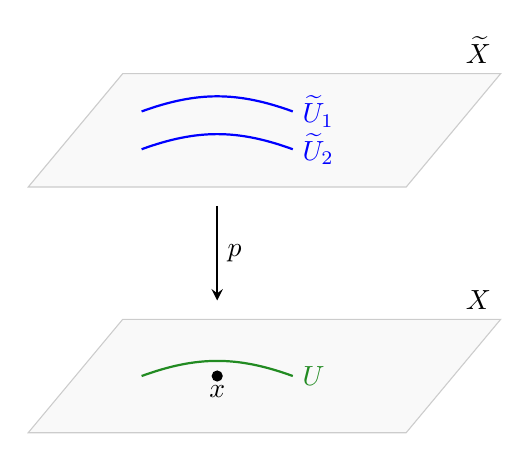
\begin{tikzpicture}[scale=1.2]
        % Espacio revestimento \widetilde{X}
        \draw[gray!40, fill=gray!5] (-2,1.8) -- (2,1.8) -- (3,3) -- (-1,3) -- cycle;
        \node[above left] at (3,3) {$\widetilde{X}$};

        % Hojas \widetilde{U}_\alpha
        \draw[thick, blue] (-0.8, 2.6) to[out=20, in=160] (0.8, 2.6);
        \node[blue, right] at (0.8, 2.6) {$\widetilde{U}_1$};
        \draw[thick, blue] (-0.8, 2.2) to[out=20, in=160] (0.8, 2.2);
        \node[blue, right] at (0.8, 2.2) {$\widetilde{U}_2$};

        % Proyección p
        \draw[->, >=stealth, thick] (0, 1.6) -- (0, 0.6) node[midway, right] {$p$};

        % Espacio base X
        \draw[gray!40, fill=gray!5] (-2,-0.8) -- (2,-0.8) -- (3,0.4) -- (-1,0.4) -- cycle;
        \node[above left] at (3,0.4) {$X$};

        % Intorno U y punto x
        \draw[thick, ForestGreen] (-0.8, -0.2) to[out=20, in=160] (0.8, -0.2);
        \node[ForestGreen, right] at (0.8, -0.2) {$U$};
        \filldraw[black] (0, -0.2) circle (1.5pt) node[below] {$x$};
    \end{tikzpicture}
    \caption{Struttura locale di uno spazio di rivestimento $p: \widetilde{X} \to X$.}
\end{figure}

\begin{prop}[Proprietà di base dei rivestimenti]
Sia $(\widetilde{X}, p)$ uno spazio di rivestimento di $X$.
\begin{enumerate}
    \item \textbf{$p$ è suriettiva:}
    Per ogni $x \in X$, sia $U$ un intorno ben coperto di $x$. Fissato un foglio $\widetilde{U}_\alpha$, poichè $p|_{\widetilde{U}_\alpha}: \widetilde{U}_\alpha \to U$ è un omeomorfismo, esiste $\widetilde{x} \in \widetilde{U}_\alpha$ tale che $p(\widetilde{x}) = x$.

    \item \textbf{$p$ è un omeomorfismo locale:}
    Per ogni $\widetilde{x} \in \widetilde{X}$, posto $x = p(\widetilde{x}) \in X$, sia $U$ un intorno ben coperto di $x$.
    Siccome $\widetilde{x} \in p^{-1}(x) \subset p^{-1}(U) = \bigsqcup \widetilde{U}_\alpha$, esiste un unico foglio $\widetilde{U}_\alpha$ contenente $\widetilde{x}$.
    L'aperto $\widetilde{U}_\alpha$ è un intorno aperto di $\widetilde{x}$ in $\widetilde{X}$ e $p|_{\widetilde{U}_\alpha}: \widetilde{U}_\alpha \to U$ è un omeomorfismo su $U = p(\widetilde{U}_\alpha)$.

    \begin{observacion}
    Ogni omeomorfismo è un omeomorfismo locale, ma il viceversa non vale in generale.
    Controesempio: La mappa $p: \mathbb{R} \to S^1$ data da $t \mapsto e^{2\pi i t}$ è un omeomorfismo locale (ed è un rivestimento), ma non è un omeomorfismo globale poichè non è iniettiva.
    \end{observacion}

    \item \textbf{La fibra $p^{-1}(x)$ è uno spazio discreto (formato da punti isolati):}
    Sia $\widetilde{x} \in p^{-1}(x)$ e sia $U$ un intorno ben coperto di $x$.
    Allora $\widetilde{x} \in \widetilde{U}_\alpha$ per un unico foglio, ed essendo $\widetilde{U}_\alpha$ aperto in $\widetilde{X}$ e $p|_{\widetilde{U}_\alpha}$ iniettiva, si ha $p^{-1}(x) \cap \widetilde{U}_\alpha = \{\widetilde{x}\}$.
    Questo prova che ogni punto della fibra è isolato.

    \item \textbf{$p$ è un'applicazione aperta:}
    Sia $\widetilde{A}$ un aperto di $\widetilde{X}$. Mostriamo che $p(\widetilde{A})$ è aperto in $X$.
    Sia $x \in p(\widetilde{A})$ e sia $U$ un intorno ben coperto di $x$.
    Esiste $\widetilde{x} \in \widetilde{A}$ tale che $p(\widetilde{x}) = x$. Poiché $\widetilde{x} \in p^{-1}(U)$, esiste un foglio $\widetilde{U}_\alpha$ contenente $\widetilde{x}$.
    
    L'intersezione $\widetilde{A} \cap \widetilde{U}_\alpha$ è un aperto di $\widetilde{U}_\alpha$.
    Essendo $p|_{\widetilde{U}_\alpha}: \widetilde{U}_\alpha \to U$ un omeomorfismo (e quindi una mappa aperta), l'immagine $p(\widetilde{A} \cap \widetilde{U}_\alpha)$ è un aperto di $U$, e quindi aperto anche in $X$.
    Inoltre $x \in p(\widetilde{A} \cap \widetilde{U}_\alpha) \subseteq p(\widetilde{A})$, il che dimostra che $p(\widetilde{A})$ è un intorno aperto di ogni suo punto, ossia $p(\widetilde{A})$ è aperto in $X$.
\end{enumerate}
\end{prop}

\begin{prop}[Aperti nel rivestimento e nella base]
Sia $p: \widetilde{X} \to X$ una applicazione continua, \textbf{aperta} e suriettiva (ad esempio una applicazione di rivestimento, per le propriet\`a 1 e 4 sopra). Per ogni $A \subseteq X$:
\[
A \text{ è aperto in } X \iff p^{-1}(A) \text{ è aperto in } \widetilde{X}.
\]
\end{prop}

\begin{proof}
($\Rightarrow$) \`E la continuit\`a di $p$. ($\Leftarrow$) Se $p^{-1}(A)$ \`e aperto, poich\'e $p$ \`e aperta e suriettiva, $A = p(p^{-1}(A))$ \`e aperto. \qedhere
\end{proof}

\begin{observacion}
L'ipotesi ``$p$ aperta'' \`e essenziale: la sola continuit\`a e suriettivit\`a non bastano (ad esempio l'identit\`a $\mathrm{id}: (\mathbb{R}, \text{discreta}) \to \mathbb{R}$ \`e continua e suriettiva, ma $p^{-1}(A)$ \`e sempre aperto, anche se $A$ non lo \`e). Negli appunti originali la proposizione era enunciata senza questa ipotesi, che per\`o veniva usata nella dimostrazione.
\end{observacion}

\begin{coro}[Teorema dell'Omeomorfismo Quoziente per i Rivestimenti]
Se $(\widetilde{X}, p)$ è uno spazio di rivestimento di $X$, allora la mappa indotta sul quoziente
\[
\widetilde{p}: \widetilde{X} / \sim_p \longrightarrow X
\]
è un \textbf{omeomorfismo}, dove $\widetilde{x} \sim_p \widetilde{y} \iff p(\widetilde{x}) = p(\widetilde{y})$. In altri termini $X$ \`e il quoziente di $\widetilde{X}$ rispetto alla relazione indotta dalle fibre di $p$.
\end{coro}
\begin{proof}
Per la proposizione, $p$ \`e una applicazione quoziente (continua, suriettiva e con la topologia di $X$ determinata da $p^{-1}$). Un'applicazione quoziente induce un omeomorfismo dal quoziente per la relazione delle sue fibre.
\end{proof}

\begin{prop}[Corrispondenza tra punti della fibra e fogli]
Sia $p: \widetilde{X} \to X$ un rivestimento, $x \in X$ e $U$ un intorno ben coperto di $x$. Esiste una corrispondenza biunivoca tra i punti della fibra $p^{-1}(x)$ e i fogli $\widetilde{U}_\alpha$ sopra $U$.
\end{prop}

\begin{proof}
Sia $p^{-1}(U) = \bigsqcup_\alpha \widetilde{U}_\alpha$. Ad ogni $\widetilde{x} \in p^{-1}(x) \subset p^{-1}(U)$ associamo l'unico foglio che lo contiene (unico perch\'e i fogli sono disgiunti). Viceversa, dato un foglio $\widetilde{U}_\alpha$, la restrizione $p|_{\widetilde{U}_\alpha}: \widetilde{U}_\alpha \to U$ \`e un omeomorfismo, quindi esiste un unico punto $\widetilde{x} \in \widetilde{U}_\alpha$ con $p(\widetilde{x}) = x$. Le due costruzioni sono una l'inversa dell'altra\hfill$\square$
\end{proof}

\section{Esempi di Spazi di Rivestimento}

\begin{ejemplo}[Rivestimento della circonferenza $S^1$ tramite la retta reale $\mathbb{R}$]
Consideriamo l'applicazione mappa esponenziale:
\Func{p}{\mathbb{R}}{S^1}{t}{e^{2\pi i t} = (\cos(2\pi t), \sin(2\pi t))}

Allora la coppia $(\mathbb{R}, p)$ è uno \textbf{spazio di rivestimento} di $S^1$ ad \textbf{infinite foglie}.

\begin{proof}
Dimostriamo le proprietà richieste:

\begin{itemize}
    \item \textbf{$p$ è continua, suriettiva ed aperta:}
    La continuità segue dalla continuità delle componenti trigonometriche. La suriettivit\`a \`e nota; l'apertura segue dal fatto che l'immagine di un intervallo aperto di lunghezza $\leqslant 1$ \`e un arco aperto di $S^1$ e ogni aperto di $\mathbb{R}$ \`e unione di tali intervalli.

    \item \textbf{Costruzione degli intorni ben coperti:}
    Fissiamo un punto $x \in S^1$ e scegliamo un punto della fibra $\widetilde{x} \in p^{-1}(x)$, con $\widetilde{x} = t \in \mathbb{R}$ tale che $x = e^{2\pi i t}$.

    Scegliamo $a, b \in \mathbb{R}$ tali che $a < t < b$ e $b - a < 1$.
    L'intervallo aperto $]a, b[$ è un intorno aperto di $t$ in $\mathbb{R}$. Poiché $p$ è un'applicazione aperta, l'immagine:
    \[
    p(]a, b[) = \wideparen{p(a)p(b)}
    \]
    è un arco aperto di $S^1$ contenente $x = p(t)$.

    \item \textbf{Verifica dell'omeomorfismo locale:}
    La restrizione $p|_{]a,b[}: ]a,b[ \to \wideparen{p(a)p(b)}$ è una bigezione continua ed aperta, quindi è un \textbf{omeomorfismo}.

    Infatti, per la continuità di $p$, la restrizione $p|_{]a,b[}$ è continua. Essendo $]a,b[$ aperto in $\mathbb{R}$ e $p$ una mappa aperta, $p|_{]a,b[}$ è aperta.
    Per l'iniettività, siano $t, t' \in ]a,b[$ tali che $p(t) = p(t')$.
    Allora $e^{2\pi i t} = e^{2\pi i t'} \implies 2\pi(t - t') \in 2\pi\mathbb{Z} \implies t - t' \in \mathbb{Z}$.
    Poiché $|t - t'| < b - a < 1$, l'unica possibilità è $t - t' = 0 \implies t = t'$.

    \item \textbf{Scomposizione della controimmagine in fogli disgiunti:}
    Osserviamo che la controimmagine dell'arco aperto $U = \wideparen{p(a)p(b)}$ si scompone nell'unione disgiunta:
    \[
    p^{-1}(U) = p^{-1}(p(]a,b[)) = \coprod_{z \in \mathbb{Z}} ]a+z, b+z[
    \]
    Per ogni $z \in \mathbb{Z}$, la traslazione $t_z: ]a,b[ \to ]a+z, b+z[$ definita da $t_z(t) = t + z$ è un omeomorfismo.

    Pertanto, la restrizione di $p$ su ciascun foglio $]a+z, b+z[$ si esprime come la composizione dell'omeomorfismo di restrizione e della traslazione:
    \[
    p|_{]a+z, b+z[} = p|_{]a,b[} \circ t_{-z}
    \]
    Essendo composizione di omeomorfismi, $p|_{]a+z, b+z[}: ]a+z, b+z[ \to U$ è un omeomorfismo per ogni $z \in \mathbb{Z}$.
\end{itemize}
\end{proof}

\begin{observacion}
L'applicazione $p: \mathbb{R} \to S^1$ data da $t \mapsto e^{2\pi i t}$ è anche un \textbf{omomorfismo di gruppi} dal gruppo additivo $(\mathbb{R}, +)$ al gruppo moltiplicativo $(S^1, \cdot)$.
Infatti, per ogni $t, t' \in \mathbb{R}$:
\[
p(t + t') = e^{2\pi i (t + t')} = e^{2\pi i t} \cdot e^{2\pi i t'} = p(t) \cdot p(t')
\]
\end{observacion}
\end{ejemplo}

\vspace{1.5em}

\begin{ejemplo}[Interpretazione Geometrica: L'Elica Cilindrica]
Sia $\mathcal{E} \subset \mathbb{R}^3$ l'elica cilindrica di equazioni parametriche:
\[
\begin{cases}
    x = \cos(2\pi t) \\
    y = \sin(2\pi t) \\
    z = t
\end{cases}
\quad t \in \mathbb{R}
\]

\begin{figure}[H]
    \centering
    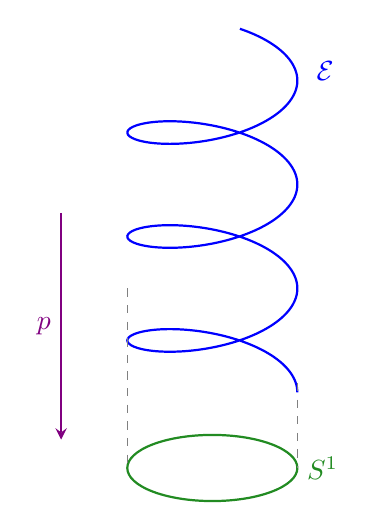
\begin{tikzpicture}[scale=1.2]
        % elica (proiezione obliqua): x = cos(2 pi t), y = sin(2 pi t), z = t
        \draw[domain=-1:2.2, samples=200, smooth, variable=\t, blue, thick]
            plot ({0.9*cos(360*\t)}, {0.35*sin(360*\t) + 1.1*\t});
        \node[blue, right] at (1.0,2.3) {$\mathcal{E}$};
        % circonferenza base
        \draw[thick, ForestGreen] (0,-1.9) ellipse (0.9cm and 0.35cm);
        \node[ForestGreen, right] at (0.9,-1.9) {$S^1$};
        \draw[dashed, gray] (0.9,-1.0) -- (0.9,-1.9);
        \draw[dashed, gray] (-0.9, 0.0) -- (-0.9,-1.9);
        \draw[->, >=stealth, thick, Purple] (-1.6, 0.8) -- (-1.6, -1.6) node[midway, left] {$p$};
    \end{tikzpicture}
    \caption{L'elica cilindrica $\mathcal{E}$ si proietta sulla circonferenza $S^1$ ``avvolgendosi'' infinite volte: ogni punto di $S^1$ ha infinite controimmagini (una per ogni giro).}
\end{figure}

Come insieme di punti, l'elica $\mathcal{E}$ è omeomorfa alla retta reale $\mathbb{R}$ tramite l'omeomorfismo $f: \mathbb{R} \to \mathcal{E}$ dato da $t \mapsto (\cos(2\pi t), \sin(2\pi t), t)$.

La proiezione verticale $p: \mathcal{E} \to S^1$ definita da $(\cos(2\pi t), \sin(2\pi t), t) \mapsto (\cos(2\pi t), \sin(2\pi t))$ corrisponde alla mappa esponenziale $t \mapsto e^{2\pi i t}$, confermando geometricamente che l'elica «srotola» la circonferenza in un rivestimento ad infinite foglie.
\end{ejemplo}

\vspace{2em}

\begin{ejemplo}[Rivestimento del Toro $n$-Dimensionale $T^n$]
Consideriamo l'applicazione proiettiva:
\Func{\overline{p}}{\mathbb{R}^n}{\underbrace{S^1 \times \dots \times S^1}_{n \text{ volte}} = T^n}{(t_1, \dots, t_n)}{(p(t_1), \dots, p(t_n))}
dove $p: \mathbb{R} \to S^1$ è la mappa esponenziale $p(t) = e^{2\pi i t}$.

Allora $(\mathbb{R}^n, \overline{p})$ è uno \textbf{spazio di rivestimento} del toro $n$-dimensionale $T^n$.

\begin{proof}
Sia $(z_1, \dots, z_n) \in S^1 \times \dots \times S^1 = T^n$.
Per ogni $r = 1, \dots, n$, scegliamo un punto $t_r \in p^{-1}(z_r)$ ed intervalli $]a_r, b_r[$ con $a_r < t_r < b_r$ e $b_r - a_r < 1$.

Consideriamo il prodotto cartesiano degli archi aperti su $T^n$:
\[
V = \overline{p}\left( ]a_1, b_1[ \times \dots \times ]a_n, b_n[ \right) = \widearc{p(a_1)p(b_1)} \times \dots \times \widearc{p(a_n)p(b_n)}
\]
$V$ è un intorno aperto ben coperto di $(z_1, \dots, z_n)$ in $T^n$.

La controimmagine $\overline{p}^{-1}(V)$ in $\mathbb{R}^n$ si decompone nell'unione disgiunta di cubi aperti traslati tramite il reticolo $\mathbb{Z}^n$:
\[
\overline{p}^{-1}(V) = \bigsqcup_{h = (h_1, \dots, h_n) \in \mathbb{Z}^n} \left( ]a_1 + h_1, b_1 + h_1[ \times \dots \times ]a_n + h_n, b_n + h_n[ \right)
\]

Per ogni $h \in \mathbb{Z}^n$, la traslazione $t_h: \prod_{r=1}^n ]a_r, b_r[ \to \prod_{r=1}^n ]a_r + h_r, b_r + h_r[$ data da $t_h(x) = x + h$ è un omeomorfismo.
Inoltre, la restrizione della proiezione sul singolo blocco traslato soddisfa:
\[
\overline{p}|_{\prod_{r=1}^n ]a_r + h_r, b_r + h_r[} = \overline{p}|_{\prod_{r=1}^n ]a_r, b_r[} \circ t_{-h}
\]
Trattandosi di composizione di omeomorfismi, ciascuna restrizione è un omeomorfismo sul prodotto aperto $V$.
Ciò prova che $(\mathbb{R}^n, \overline{p})$ è un rivestimento di $T^n$\hfill$\square$
\end{proof}
\end{ejemplo}

\vspace{2em}

\section{Lo Spazio Proiettivo Reale e il suo Rivestimento tramite $S^n$}

\begin{definicion}[Spazio Proiettivo Reale $\mathbb{R}P^n$]
Consideriamo lo spazio vettoriale $\mathbb{R}^{n+1} \setminus \{\bar{0}\}$.
Definiamo la seguente relazione di equivalenza $\sim$ su $\mathbb{R}^{n+1} \setminus \{\bar{0}\}$:
\[
x \sim y \iff \exists t \in \mathbb{R} \setminus \{0\} \text{ tale che } y = t x
\]
Lo \textbf{spazio proiettivo reale} di dimensione $n$ è lo spazio topologico quoziente:
\[
\mathbb{R}P^n = \left( \mathbb{R}^{n+1} \setminus \{\bar{0}\} \right) \big/ \sim
\]
ovvero l'insieme di tutte le rette passanti per l'origine in $\mathbb{R}^{n+1}$ dotate della topologia quoziente. Indichiamo con
\Func{\pi}{\mathbb{R}^{n+1} \setminus \{\bar{0}\}}{\mathbb{R}P^n}{x}{[x]_\sim = \{t x \mid t \neq 0\}}
la proiezione canonica (continua per definizione di topologia quoziente).
\end{definicion}

\section{Proprietà dello Spazio Proiettivo Reale $\mathbb{R}P^n$}

\begin{prop}
$\mathbb{R}P^n$ è uno spazio connesso (e connesso per archi).
\end{prop}

\begin{proof}
Essendo $\mathbb{R}P^n = \pi\left(\mathbb{R}^{n+1} \setminus \{\bar{0}\}\right)$ l'immagine continua dello spazio $\mathbb{R}^{n+1} \setminus \{\bar{0}\}$, ed essendo quest'ultimo connesso per archi per ogni $n \geqslant 1$ (e $\pi$ continua), ne consegue che $\mathbb{R}P^n$ è connesso per archi.
\end{proof}

\begin{prop}
$\mathbb{R}P^n$ è uno spazio di Hausdorff ($T_2$).
\end{prop}

\begin{proof}
Sia $\mathcal{C}$ un cono aperto di vertice $\bar{0}$ in $\mathbb{R}^{n+1} \setminus \{\bar{0}\}$.
Osserviamo che per ogni $x \in \mathcal{C}$, l'intera retta vettoriale privata dell'origine è contenuta in $\mathcal{C}$, ossia $\pi^{-1}(\pi(\mathcal{C})) = \mathcal{C}$.
Definiamo $\overline{\mathcal{C}} = \pi(\mathcal{C})$. Per la definizione di topologia quoziente, un insieme $A \subseteq \mathbb{R}P^n$ è aperto se e solo se $\pi^{-1}(A)$ è un aperto di $\mathbb{R}^{n+1} \setminus \{\bar{0}\}$.
Essendo $\pi^{-1}(\overline{\mathcal{C}}) = \mathcal{C}$ un cono aperto, $\overline{\mathcal{C}}$ è un aperto di $\mathbb{R}P^n$.

\begin{figure}[H]
    \centering
    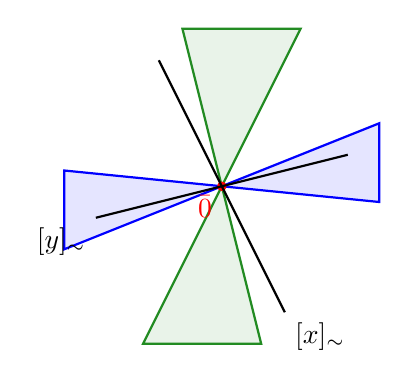
\begin{tikzpicture}[scale=1.0]
        % Conos abiertos en R^{n+1}
        \draw[thick, ForestGreen, fill=ForestGreen!10] (0,0) -- (1,2) -- (-0.5,2) -- cycle;
        \draw[thick, ForestGreen, fill=ForestGreen!10] (0,0) -- (-1,-2) -- (0.5,-2) -- cycle;
        
        \draw[thick, blue, fill=blue!10] (0,0) -- (2,0.8) -- (2,-0.2) -- cycle;
        \draw[thick, blue, fill=blue!10] (0,0) -- (-2,-0.8) -- (-2,0.2) -- cycle;

        \filldraw[red] (0,0) circle (1.5pt) node[below left] {$\bar{0}$};
        
        % Ejes/Rettas
        \draw[thick] (-0.8,1.6) -- (0.8,-1.6) node[below right] {$[x]_\sim$};
        \draw[thick] (1.6,0.4) -- (-1.6,-0.4) node[below left] {$[y]_\sim$};
    \end{tikzpicture}
    \caption{Separazione di due rette distinte tramite coni aperti disgiunti in $\mathbb{R}^{n+1}$.}
\end{figure}

Siano ora $[x]_\sim, [y]_\sim \in \mathbb{R}P^n$ due punti distinti con $[x]_\sim \neq [y]_\sim$, il che equivale a dire che le rette vettoriali ordinate da $x$ e $y$ sono distinte.
Possiamo scegliere due coni aperti $\mathcal{C}_1$ e $\mathcal{C}_2$ di assi $[x]_\sim$ e $[y]_\sim$ rispettivamente, tali che $\mathcal{C}_1 \cap \mathcal{C}_2 = \varnothing$. Esplicitamente: siano $u = x/\|x\|$, $w = y/\|y\|$; poich\'e le rette sono distinte, $d = \min\{\|u - w\|, \|u + w\|\} > 0$. Posto $\delta = d/2$ e
\[
\mathcal{C}_1 = \Big\{ v \neq \bar 0 \;:\; \min\big\|\tfrac{v}{\|v\|} \mp u\big\| < \delta \Big\}, \qquad
\mathcal{C}_2 = \Big\{ v \neq \bar 0 \;:\; \min\big\|\tfrac{v}{\|v\|} \mp w\big\| < \delta \Big\},
\]
i due insiemi sono aperti, invarianti per moltiplicazione per scalari non nulli (coni), contengono rispettivamente le rette di $x$ e $y$, e sono disgiunti: se $v$ stesse in entrambi, per la disuguaglianza triangolare $\|\pm u \mp w\| < 2\delta = d$, assurdo.

Ma allora le loro immagini $\overline{\mathcal{C}}_1 = \pi(\mathcal{C}_1)$ e $\overline{\mathcal{C}}_2 = \pi(\mathcal{C}_2)$ sono intorni aperti disgiunti di $[x]_\sim$ e $[y]_\sim$ in $\mathbb{R}P^n$, ovvero $\overline{\mathcal{C}}_1 \cap \overline{\mathcal{C}}_2 = \varnothing$.
Questo dimostra che $\mathbb{R}P^n$ soddisfa l'assioma $T_2$\hfill$\square$
\end{proof}

\vspace{1.5em}

\begin{prop}
Consideriamo la sfera unitaria $S^n \subset \mathbb{R}^{n+1} \setminus \{\bar{0}\}$ e la restrizione della proiezione canonica:
\Func{p = \pi|_{S^n}}{S^n}{\mathbb{R}P^n}{x}{[x]_\sim}
Allora $(S^n, p)$ è uno \textbf{spazio di rivestimento a 2 foglie} di $\mathbb{R}P^n$.
\end{prop}

\begin{coro}
Lo spazio proiettivo reale è omeomorfo al quoziente della sfera rispetto all'azione dei punti antipodali:
\[
\mathbb{R}P^n \cong S^n \big/ \{ \pm \mathrm{Id}_{S^n} \}
\]
\end{coro}

\begin{proof}
Sia $p: S^n \to \mathbb{R}P^n$ la mappa di rivestimento a 2 foglie. Due punti $x, x' \in S^n$ soddisfano $p(x) = p(x')$ se e solo se $x' = \pm x$ (punti antipodali).
Dato che la relazione indotta dal rivestimento identifica ogni punto con il suo antipodo ($x \sim_p x' \iff x' = \pm x$), dal Teorema dell'Omeomorfismo Quoziente segue che:
\[
\mathbb{R}P^n = S^n \big/ \sim_p \;\;\cong\;\; S^n \big/ \{ \pm \mathrm{Id}_{S^n} \}
\]
\end{proof}

\begin{coro}
Lo spazio proiettivo reale $\mathbb{R}P^n$ è uno spazio topologico \textbf{compatto}.
\end{coro}

\begin{proof}
$\mathbb{R}P^n = p(S^n)$ è l'immagine continua della sfera unitaria $S^n$, la quale è un sottoinsieme chiuso e limitato di $\mathbb{R}^{n+1}$, e quindi compatta per il Teorema di Heine-Borel.
\end{proof}

\vspace{2em}

\section{Esempi Notevoli di Spazi Proiettivi Reali}

\begin{ejemplo}[Caso $n=1$: $\mathbb{R}P^1 \cong S^1$]
Dimostriamo che la retta proiettiva reale è omeomorfa alla circonferenza $S^1$.

\begin{proof}
Rappresentiamo la circonferenza come l'insieme dei numeri complessi di modulo unitario $S^1 = \{z \in \mathbb{C} \mid |z| = 1\}$. Ogni elemento $z \in S^1$ si scrive nella forma $z = e^{i\theta}$ con $\theta \in \mathbb{R}$.

Consideriamo l'applicazione di elevamento al quadrato $f: S^1 \to S^1$ definita da:
\[
f(z) = z^2 = e^{2i\theta}
\]
$f$ è ben posta, continua e suriettiva.

\begin{itemize}
    \item \textbf{$f$ è un'applicazione aperta:}
    Sia $\widearc{a,b}$ un arco aperto su $S^1$. L'immagine $f(\widearc{a,b})$ corrisponde all'arco duplicato $\widearc{a^2, b^2}$. Se la lunghezza dell'arco iniziale supera $\pi$, l'immagine ricopre l'intera circonferenza $S^1$ (che è aperta), altrimenti produce un arco aperto.

    \item \textbf{Relazione di equivalenza indotta:}
    Per ogni $z, z' \in S^1$, si ha:
    \[
    f(z) = f(z') \iff z^2 = (z')^2 \iff z' = \pm z
    \]
    Quindi la relazione indotta da $f$ identifica esattamente i punti antipodali di $S^1$.
\end{itemize}

Poich\'e $f$ \`e continua, aperta e suriettiva, essa \`e una applicazione quoziente, quindi induce un omeomorfismo
\[
\widetilde{f}: S^1 \big/ \sim_f \;=\; S^1 \big/ \{ \pm \mathrm{Id}_{S^1} \} \xrightarrow{\ \cong\ } S^1 .
\]
D'altra parte, per il corollario sul rivestimento $S^n \to \mathbb{R}P^n$ (con $n=1$), $S^1 / \{\pm \mathrm{Id}\} \cong \mathbb{R}P^1$. Componendo, $\mathbb{R}P^1 \cong S^1$\hfill$\square$
\end{proof}
\end{ejemplo}

\vspace{1.5em}

\begin{ejemplo}[Caso $n=2$: Il Piano Proiettivo Reale $\mathbb{R}P^2$]
Analizziamo la rappresentazione topologica del piano proiettivo reale $\mathbb{R}P^2 = S^2 / \{ \pm \mathrm{Id} \}$.

\begin{figure}[H]
    \centering
    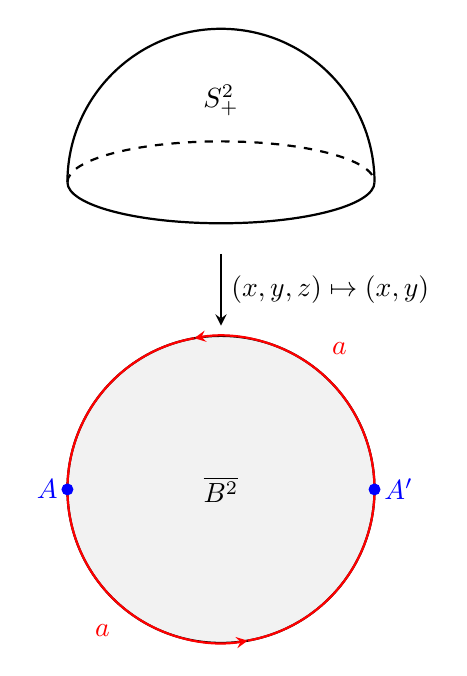
\begin{tikzpicture}[scale=1.3]
        % emisfero superiore
        \draw[thick] (-1.5,0) arc (180:0:1.5);
        \draw[thick] (-1.5,0) arc (180:360:1.5 and 0.4);
        \draw[thick, dashed] (-1.5,0) arc (180:0:1.5 and 0.4);
        \node at (0,0.8) {$S^2_+$};
        \draw[->, >=stealth, thick] (0,-0.7) -- (0,-1.4) node[midway, right] {$(x,y,z) \mapsto (x,y)$};
        % disco
        \begin{scope}[shift={(0,-3.0)}]
            \draw[thick, fill=gray!10] (0,0) circle (1.5cm);
            \node at (0,0) {$\overline{B^2}$};
            \draw[thick, red, ->, >=stealth] (0:1.5) arc (0:100:1.5);
            \draw[thick, red] (100:1.5) arc (100:180:1.5);
            \draw[thick, red, ->, >=stealth] (180:1.5) arc (180:280:1.5);
            \draw[thick, red] (280:1.5) arc (280:360:1.5);
            \node[red] at (50:1.8) {$a$};
            \node[red] at (230:1.8) {$a$};
            \filldraw[blue] (0:1.5) circle (1.5pt) node[right] {$A'$};
            \filldraw[blue] (180:1.5) circle (1.5pt) node[left] {$A$};
        \end{scope}
    \end{tikzpicture}
    \caption{$S^2_+ \cong \overline{B^2}$ tramite la proiezione ortogonale; sul bordo si identificano i punti antipodali (i due semicerchi, entrambi percorsi in senso antiorario, sono identificati: parola $aa$).}
\end{figure}

Consideriamo l'emisfero superiore chiuso della sfera 2-dimensionale:
\[
S^2_+ = \left\{ (x,y,z) \in \mathbb{R}^3 \;\middle|\; x^2 + y^2 + z^2 = 1, \; z \geqslant 0 \right\}
\]

Ogni punto dell'emisfero inferiore $S^2_-$ ha un unico punto antipodale nell'emisfero superiore $S^2_+$. L'unica sovrapposizione avviene sull'equatore $z=0$, dove i punti antipodali si trovano sul bordo $\partial S^2_+ \cong S^1$. Inoltre $p|_{S^2_+}: S^2_+ \to \mathbb{R}P^2$ \`e continua e suriettiva da uno spazio compatto a uno spazio di Hausdorff, quindi \`e chiusa e dunque una applicazione quoziente; le sue fibre sono i singoli punti di $S^2_+$ con $z>0$ e le coppie di punti antipodali dell'equatore.

L'applicazione di proiezione ortogonale $f: S^2_+ \to \overline{B^2}$ definita da $f(x,y,z) = (x,y)$ è un \textbf{omeomorfismo} tra l'emisfero superiore $S^2_+$ ed il disco chiuso bidimensionale $\overline{B^2}$.

Pertanto, il piano proiettivo reale $\mathbb{R}P^2$ è topologicamente equivalente al \textbf{disco chiuso $\overline{B^2}$ con i punti antipodali del bordo $\partial B^2 = S^1$ identificati a due a due}:
\[
\mathbb{R}P^2 \cong \overline{B^2} \big/ \sim_{\text{antipodale su } \partial B^2}
\]
\end{ejemplo}

\section{Modelli topologici di $\mathbb{R}P^n$}

\begin{teo}
Lo spazio proiettivo reale $\mathbb{R}P^2$ è omeomorfo al quoziente del disco chiuso bidimensionale:
\[
\mathbb{R}P^2 \cong \overline{B^2} \big/ \sim
\]
dove $\sim$ è la relazione di equivalenza su $\overline{B^2}$, non banale solo sul bordo $\partial \overline{B^2} \cong S^1$, che identifica a due a due i punti antipodali di $\partial \overline{B^2}$.
\end{teo}

\vspace{1em}

\begin{prop}[Generalizzazione in dimensione $n$]
Per ogni $n \geqslant 1$, lo spazio proiettivo reale $\mathbb{R}P^n$ soddisfa:
\[
\mathbb{R}P^n = S^n \big/ \{\pm \mathrm{Id}\} = S^n \big/ \sim \;\;\cong\;\; \overline{B^n} \big/ \sim
\]
dove $\sim$ è la relazione di equivalenza su $\overline{B^n}$, non banale solo sul bordo $\partial \overline{B^n} = S^{n-1}$, che ne identifica a due a due i punti antipodali.
\end{prop}

\begin{proof}[Dimostrazione (per ogni $n \geqslant 1$, in particolare $n=2$ del teorema precedente)]
Sia $S^n_+ = \{x \in S^n \mid x_{n+1} \geqslant 0\}$. Ogni retta per l'origine incontra $S^n_+$ (se $x_{n+1} < 0$ si usa $-x$), e la incontra in due punti (antipodali) solo se sta nell'iperpiano $x_{n+1} = 0$, cio\`e se i punti sono sul bordo $\partial S^n_+ = S^{n-1}$. Dunque $p|_{S^n_+}: S^n_+ \to \mathbb{R}P^n$ \`e continua e suriettiva, con fibre ``banali'' fuori dal bordo e coppie antipodali sul bordo. Essendo $S^n_+$ compatto e $\mathbb{R}P^n$ di Hausdorff, $p|_{S^n_+}$ \`e chiusa, quindi quoziente: $\mathbb{R}P^n \cong S^n_+/\!\sim$. Infine la proiezione $(x_1, \dots, x_{n+1}) \mapsto (x_1, \dots, x_n)$ \`e un omeomorfismo $S^n_+ \to \overline{B^n}$ (inversa $y \mapsto (y, \sqrt{1-\|y\|^2})$) che manda $\partial S^n_+$ in $\partial \overline{B^n} = S^{n-1}$ e rispetta l'identificazione antipodale\hfill$\square$
\end{proof}

\begin{ejercicio*}[\textbf{DOMANDA D'ESAME}]
\textbf{Quali sono i modelli topologici di $\mathbb{R}P^n$?}
\begin{enumerate}
    \item Il quoziente dello spazio vettoriale: $\left(\mathbb{R}^{n+1} \setminus \{\bar{0}\}\right) / \sim$.
    \item Il quoziente della sfera unitaria per l'azione antipodale: $S^n / \{\pm \mathrm{Id}_{S^n}\}$.
    \item Il quoziente del disco chiuso con identificazione antipodale sul bordo: $\overline{B^n} / \sim$.
\end{enumerate}
\end{ejercicio*}

\vspace{2em}

\section{Dimostrazione: $(S^n, p)$ \`e un rivestimento di $\mathbb{R}P^n$}

\begin{teo}
La coppia $(S^n, p)$, con $p = \pi|_{S^n}: S^n \to \mathbb{R}P^n$, è uno \textbf{spazio di rivestimento a 2 foglie} dello spazio proiettivo reale $\mathbb{R}P^n$.
\end{teo}

\begin{proof}
Dimostriamo le proprietà fondamentali della mappa di rivestimento $p$:

\begin{itemize}
    \item \textbf{$p$ è continua:}
    La mappa $p = \pi|_{S^n}$ è la restrizione alla sfera della proiezione canonica $\pi: \mathbb{R}^{n+1} \setminus \{\bar{0}\} \to \mathbb{R}P^n$, che è continua per definizione di topologia quoziente.

    \item \textbf{$p$ è suriettiva:}
    Sia $[y]_\sim \in \mathbb{R}P^n$, con $y \in \mathbb{R}^{n+1} \setminus \{\bar{0}\}$.
    Normalizziamo il vettore ponendo $x = \frac{y}{\|y\|} \in S^n$.
    Allora l'immagine tramite $p$ è $p(x) = \pi(x) = \pi\left(\frac{y}{\|y\|}\right) = \pi(y) = [y]_\sim$.

    \item \textbf{Caratterizzazione della fibra:}
    Per ogni $x, x' \in S^n$, mostriamo che $p(x) = p(x') \iff x' = \pm x$.
    \begin{itemize}
        \item[$\impliedby$)] Banale: se $x' = \pm x \implies [x']_\sim = [x]_\sim \implies p(x') = p(x)$.
        \item[$\implies$)] Se $p(x) = p(x')$, allora $[x]_\sim = [x']_\sim$, il che implica che esiste $t \neq 0$ tale che $x' = t x$.
        Passando alle norme euclidee:
        \[
        1 = \|x'\| = \|t x\| = |t| \cdot \|x\| = |t| \implies t = \pm 1 \implies x' = \pm x
        \]
    \end{itemize}
    Di conseguenza, per ogni $[y]_\sim \in \mathbb{R}P^n$, la fibra $p^{-1}([y]_\sim)$ contiene esattamente due punti antipodali:
    \[
    p^{-1}([y]_\sim) = \left\{ \frac{y}{\|y\|}, \, -\frac{y}{\|y\|} \right\}
    \]
\end{itemize}

\begin{figure}[H]
    \centering
    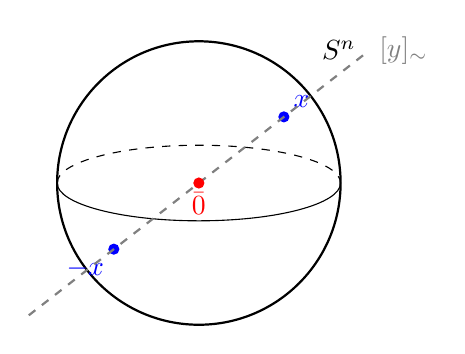
\begin{tikzpicture}[scale=1.2]
        % Sfera S^n
        \draw[thick] (0,0) circle (1.5cm);
        \draw[dashed] (-1.5,0) arc (180:0:1.5cm and 0.4cm);
        \draw (-1.5,0) arc (180:360:1.5cm and 0.4cm);
        \node[above right] at (1.2,1.2) {$S^n$};

        % Punti antipodali
        \filldraw[blue] (0.9, 0.7) circle (1.5pt) node[above right] {$x$};
        \filldraw[blue] (-0.9, -0.7) circle (1.5pt) node[below left] {$-x$};
        
        % Retta per l'origine
        \draw[thick, gray, dashed] (-1.8,-1.4) -- (1.8,1.4) node[right] {$[y]_\sim$};
        \filldraw[red] (0,0) circle (1.5pt) node[below] {$\bar{0}$};
    \end{tikzpicture}
    \caption{Intersezione della retta vettoriale $[y]_\sim$ con la sfera $S^n$ nei punti antipodali $\pm x$.}
\end{figure}

\begin{itemize}
    \item \textbf{Costruzione degli intorni ben coperti.} Sia $[y]_\sim \in \mathbb{R}P^n$ e $x = y/\|y\|$. Poniamo
    \[
    V = \{ [v]_\sim \;:\; \langle v, x \rangle \neq 0 \} \subseteq \mathbb{R}P^n .
    \]
    La condizione $\langle v,x\rangle \neq 0$ \`e invariante per $v \mapsto tv$, e $\pi^{-1}(V) = \{v : \langle v, x\rangle \neq 0\}$ \`e aperto; quindi $V$ \`e un intorno aperto di $[y]_\sim$ (contiene $[x]_\sim$). La sua controimmagine in $S^n$ \`e l'unione disgiunta di due emisferi aperti
    \[
    p^{-1}(V) = \widetilde{U}_+ \sqcup \widetilde{U}_-, \qquad \widetilde{U}_\pm = \{ z \in S^n : \pm\langle z, x \rangle > 0 \},
    \]
    antipodali tra loro ($\widetilde{U}_- = -\widetilde{U}_+$), aperti in $S^n$ e disgiunti.

    Mostriamo che $p|_{\widetilde{U}_+}: \widetilde{U}_+ \to V$ \`e un omeomorfismo (per $\widetilde{U}_-$ \`e identico).
    \begin{enumerate}[label=\roman*)]
        \item \`E continua (restrizione di $p$) e \textbf{iniettiva}: se $p(z) = p(z')$ con $z, z' \in \widetilde{U}_+$, allora $z' = \pm z$; ma $-z \in \widetilde{U}_-$, quindi $z' = z$.
        \item \`E \textbf{suriettiva}: se $[v]_\sim \in V$, allora $\langle v, x \rangle \neq 0$ e il punto $z = \operatorname{sgn}\langle v,x\rangle \, v/\|v\|$ sta in $\widetilde{U}_+$ e $p(z) = [v]_\sim$.
        \item L'\textbf{inversa} $V \to \widetilde{U}_+$ \`e continua. Sia $s: \pi^{-1}(V) \to \widetilde{U}_+$ data da $s(v) = \operatorname{sgn}\langle v,x\rangle\, v/\|v\|$: \`e continua (il segno \`e localmente costante su $\pi^{-1}(V)$) e costante sulle fibre di $\pi$, perch\'e $s(tv) = s(v)$ per ogni $t \neq 0$. Poich\'e $\pi|_{\pi^{-1}(V)}: \pi^{-1}(V) \to V$ \`e una applicazione quoziente (restrizione di un quoziente a un aperto saturo), $s$ induce una applicazione continua $V \to \widetilde{U}_+$, che \`e proprio $(p|_{\widetilde{U}_+})^{-1}$.
    \end{enumerate}
    Quindi ciascun $\widetilde{U}_\pm$ \`e un foglio omeomorfo a $V$ tramite $p$. (Inoltre $S^n$ \`e connessa per archi per $n \geqslant 1$, come richiesto dalla definizione di rivestimento.)
\end{itemize}
In conclusione, $(S^n, p)$ è uno spazio di rivestimento a 2 foglie di $\mathbb{R}P^n$\hfill$\square$
\end{proof}

% ======== NUOVO (pp. 89-92 degli appunti, 13/10/2026) ========
\section{Altri esempi di rivestimenti e sollevamenti}

\begin{ejemplo}[Rivestimenti del toro]
\begin{enumerate}
    \item L'applicazione
    \Func{p}{\mathbb{R} \times S^1}{S^1 \times S^1 = T^2}{(x,z)}{(e^{2\pi i x},\, z)}
    \`e un'applicazione di rivestimento del toro $T^2$ tramite il \emph{cilindro} $\mathbb{R} \times S^1$ (si ``avvolge'' soltanto la prima circonferenza).
    \item Anche l'applicazione
    \Func{p}{\mathbb{R}^2 = \mathbb{R} \times \mathbb{R}}{\mathbb{R} \times S^1}{(x,y)}{(x,\, e^{2\pi i y})}
    \`e un rivestimento (del cilindro).
\end{enumerate}
\end{ejemplo}

\begin{observacion}
Il rivestimento di uno spazio $X$ \textbf{non \`e unico}: sia $\mathbb{R}^2$ sia il cilindro $\mathbb{R} \times S^1$ sono rivestimenti di $T^2$ (il primo tramite $(x,y) \mapsto (e^{2\pi i x}, e^{2\pi i y})$, il secondo come sopra). Il rivestimento $\mathbb{R}^2 \to T^2$ ``srotola'' entrambe le circonferenze, quello dal cilindro ne srotola una sola.
\end{observacion}

\begin{figure}[H]
    \centering
    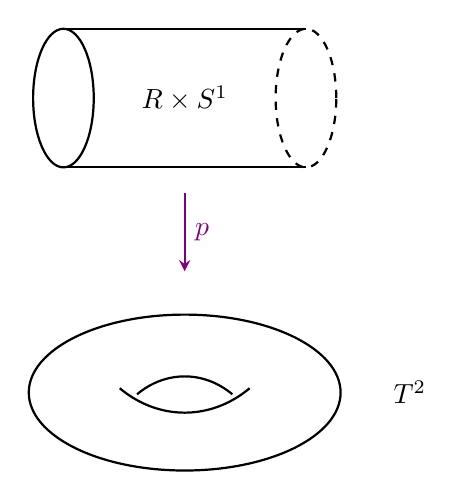
\begin{tikzpicture}[scale=1.1]
        % cilindro
        \draw[thick] (-1.2,0) ellipse (0.35 and 0.8);
        \draw[thick] (-1.2,0.8) -- (1.6,0.8);
        \draw[thick] (-1.2,-0.8) -- (1.6,-0.8);
        \draw[thick, dashed] (1.6,0) ellipse (0.35 and 0.8);
        \node at (0.2,0) {$\mathbb{R} \times S^1$};
        \draw[->, >=stealth, thick, Purple] (0.2,-1.1) -- (0.2,-2.0) node[midway, right] {$p$};
        % toro (schematico)
        \begin{scope}[shift={(0.2,-3.4)}]
            \draw[thick] (0,0) ellipse (1.8 and 0.9);
            \draw[thick] (-0.75,0.05) to[bend right=40] (0.75,0.05);
            \draw[thick] (-0.55,-0.02) to[bend left=40] (0.55,-0.02);
            \node at (2.6,0) {$T^2$};
        \end{scope}
    \end{tikzpicture}
    \caption{Il cilindro $\mathbb{R}\times S^1$ si avvolge sul toro $T^2$ lungo la direzione di $\mathbb{R}$.}
\end{figure}

\section{Sollevamenti}

\begin{definicion}[Sollevamento]
Sia $(\widetilde{X}, p)$ uno spazio di rivestimento di $X$, $Y$ uno spazio topologico e $f: Y \to X$ continua. Un'applicazione continua $\widetilde{f}: Y \to \widetilde{X}$ si dice \textbf{sollevamento} di $f$ se $p \circ \widetilde{f} = f$, cio\`e se il seguente diagramma commuta:
\begin{center}
\begin{tikzcd}
 & \widetilde{X} \arrow[d, "p"] \\
Y \arrow[ur, dashed, "\widetilde{f}"] \arrow[r, "f"'] & X
\end{tikzcd}
\end{center}
\end{definicion}

\begin{intuizione}
Sollevare $f$ significa ``scegliere con continuit\`a'' una controimmagine, nella fibra di $p$, del punto $f(y)$ per ogni $y \in Y$. Il teorema seguente dice che, una volta scelta la controimmagine in un punto, la scelta in tutti gli altri punti (se $Y$ \`e connesso) \`e obbligata.
\end{intuizione}

\begin{teo}[Unicit\`a del sollevamento]
Sia $(\widetilde{X}, p)$ uno spazio di rivestimento di $X$, $Y$ uno spazio topologico \textbf{connesso} e $f: Y \to X$ continua. Siano $\widetilde{f}_1, \widetilde{f}_2: Y \to \widetilde{X}$ due sollevamenti di $f$ (cio\`e $p \circ \widetilde{f}_1 = p \circ \widetilde{f}_2 = f$). Se esiste $y_0 \in Y$ tale che $\widetilde{f}_1(y_0) = \widetilde{f}_2(y_0)$, allora $\widetilde{f}_1 = \widetilde{f}_2$.
\end{teo}

\begin{proof}
Poniamo $Z = \{ y \in Y \mid \widetilde{f}_1(y) = \widetilde{f}_2(y) \}$. Vogliamo mostrare che $Z$ \`e non vuoto, aperto e chiuso: essendo $Y$ connesso, seguir\`a $Z = Y$.

\begin{itemize}
    \item \textbf{$Z \neq \varnothing$:} $y_0 \in Z$ per ipotesi.
    \item \textbf{$Z$ \`e aperto.} Sia $y \in Z$ e sia $U$ un intorno aperto ben coperto di $f(y) = p(\widetilde{f}_1(y)) \in X$. Sia $W$ l'unico foglio su $U$ contenente $\widetilde{f}_1(y) = \widetilde{f}_2(y)$. Poniamo $V = \widetilde{f}_1^{-1}(W) \cap \widetilde{f}_2^{-1}(W)$: \`e un aperto di $Y$ che contiene $y$. Se $y' \in V$, allora $\widetilde{f}_1(y'), \widetilde{f}_2(y') \in W$ e $p(\widetilde{f}_1(y')) = f(y') = p(\widetilde{f}_2(y'))$; poich\'e $p|_W: W \to U$ \`e un omeomorfismo (in particolare iniettiva), $\widetilde{f}_1(y') = \widetilde{f}_2(y')$, ossia $y' \in Z$. Dunque $V \subseteq Z$ e $Z$ \`e intorno di ogni suo punto.
    \item \textbf{$Z$ \`e chiuso} (cio\`e $Y \setminus Z$ \`e aperto). Sia $y \notin Z$: $\widetilde{f}_1(y) \neq \widetilde{f}_2(y)$, ma $p(\widetilde{f}_1(y)) = f(y) = p(\widetilde{f}_2(y))$, cio\`e i due punti stanno nella stessa fibra. Sia $U$ un intorno aperto ben coperto di $f(y)$ e siano $W_1, W_2$ i fogli su $U$ contenenti rispettivamente $\widetilde{f}_1(y)$ e $\widetilde{f}_2(y)$. Poich\'e $p$ \`e iniettiva su ciascun foglio e i due punti sono distinti con la stessa immagine, appartengono a fogli \emph{distinti}, quindi $W_1 \cap W_2 = \varnothing$. Posto $V = \widetilde{f}_1^{-1}(W_1) \cap \widetilde{f}_2^{-1}(W_2)$, aperto contenente $y$, per ogni $y' \in V$ si ha $\widetilde{f}_1(y') \in W_1$ e $\widetilde{f}_2(y') \in W_2$, che sono disgiunti: $\widetilde{f}_1(y') \neq \widetilde{f}_2(y')$. Dunque $V \subseteq Y \setminus Z$.
\end{itemize}
Per la connessione di $Y$ si conclude $Z = Y$, cio\`e $\widetilde{f}_1 = \widetilde{f}_2$\hfill$\square$
\end{proof}

\begin{observacion}
L'ipotesi di connessione \`e essenziale: se $Y = \{a\} \sqcup \{b\}$ \`e discreto e $f$ costante su $X = S^1$, si possono sollevare $a$ e $b$ in due punti diversi di una stessa fibra di $\mathbb{R} \to S^1$ senza alcun legame tra loro.
\end{observacion}


% ======== NUOVO (pp. 93-100 degli appunti) ========
\begin{coro}
Sia $(\widetilde{X}, p)$ uno spazio di rivestimento di $X$ e sia $h: \widetilde{X} \to \widetilde{X}$ continua con $p \circ h = p$. Se esiste $\widetilde{x}_0 \in \widetilde{X}$ con $h(\widetilde{x}_0) = \widetilde{x}_0$, allora $h = \mathrm{Id}_{\widetilde{X}}$.
\end{coro}

\begin{proof}
$\widetilde{X}$ \`e connesso per archi per definizione. Le applicazioni $h$ e $\mathrm{Id}_{\widetilde{X}}$ sono entrambe sollevamenti di $p: \widetilde{X} \to X$ (infatti $p \circ h = p = p \circ \mathrm{Id}_{\widetilde{X}}$) e coincidono in $\widetilde{x}_0$. Per il teorema di unicit\`a del sollevamento (con $Y = \widetilde{X}$ connesso), $h = \mathrm{Id}_{\widetilde{X}}$\hfill$\square$
\end{proof}

\begin{intuizione}
Una ``simmetria'' del rivestimento (un omeomorfismo $h$ di $\widetilde{X}$ che rispetta le fibre) che fissa anche un solo punto \`e necessariamente l'identit\`a: \`e rigidamente determinata dal valore in un punto.
\end{intuizione}

\section{Sollevamento di cammini e di omotopie}

\begin{teo}[Sollevamento dei cammini]
Sia $(\widetilde{X}, p)$ uno spazio di rivestimento di $X$, $x_0 \in X$ e $\widetilde{x}_0 \in p^{-1}(x_0)$. Se $\alpha: I \to X$ \`e un cammino con $\alpha(0) = x_0$, allora esiste un \textbf{unico} cammino $\widetilde{\alpha}: I \to \widetilde{X}$ tale che
\[
p \circ \widetilde{\alpha} = \alpha \qquad \text{e} \qquad \widetilde{\alpha}(0) = \widetilde{x}_0 .
\]
($\widetilde{\alpha}$ \`e detto \textbf{sollevamento} di $\alpha$ \emph{uscente da} $\widetilde{x}_0$.)
\end{teo}

\begin{figure}[H]
    \centering
    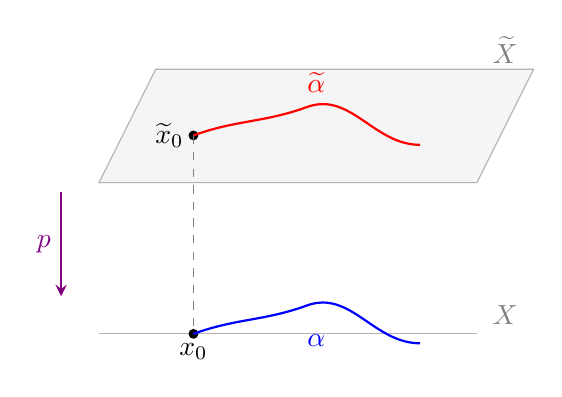
\begin{tikzpicture}[scale=1.2]
        \draw[gray!60, fill=gray!8] (-0.4,1.6) -- (3.6,1.6) -- (4.2,2.8) -- (0.2,2.8) -- cycle;
        \node[gray] at (3.9,3.0) {$\widetilde{X}$};
        \draw[gray!60] (-0.4,0) -- (3.6,0);
        \node[gray] at (3.9,0.2) {$X$};
        \filldraw (0.6,2.1) circle (1.3pt) node[left] {$\widetilde{x}_0$};
        \draw[thick, red] (0.6,2.1) to[out=20, in=200] (1.8,2.4) to[out=20, in=180] (3.0,2.0);
        \node[red, above] at (1.9,2.45) {$\widetilde{\alpha}$};
        \filldraw (0.6,0) circle (1.3pt) node[below] {$x_0$};
        \draw[thick, blue] (0.6,0) to[out=20, in=200] (1.8,0.3) to[out=20, in=180] (3.0,-0.1);
        \node[blue, below] at (1.9,0.1) {$\alpha$};
        \draw[->, >=stealth, thick, Purple] (-0.8,1.5) -- (-0.8,0.4) node[midway, left] {$p$};
        \draw[dashed, gray] (0.6,2.1) -- (0.6,0);
    \end{tikzpicture}
    \caption{Il cammino $\alpha$ in $X$ si solleva, in modo unico, a un cammino $\widetilde{\alpha}$ in $\widetilde{X}$ che parte dal punto prescelto $\widetilde{x}_0$ della fibra.}
\end{figure}

\begin{proof}
\textbf{Unicit\`a.} Segue dal teorema di unicit\`a del sollevamento, con $Y = I$ connesso: due sollevamenti di $\alpha$ uscenti da $\widetilde{x}_0$ coincidono in $0$, dunque coincidono.

\textbf{Esistenza.}
\begin{itemize}
    \item[\textbf{I passo.}] Supponiamo che esista un intorno aperto ben coperto $U$ di $x_0$ in $X$ con $\alpha(I) \subseteq U$. Sia $W$ l'unico foglio su $U$ contenente $\widetilde{x}_0$; allora $p|_W: W \to U$ \`e un omeomorfismo. Poniamo
    \[
    \widetilde{\alpha} = (p|_W)^{-1} \circ \alpha : I \to W \subseteq \widetilde{X} .
    \]
    \`E continua (composizione di continue), $p \circ \widetilde{\alpha} = p \circ (p|_W)^{-1} \circ \alpha = \alpha$ e $\widetilde{\alpha}(0) = (p|_W)^{-1}(x_0) = \widetilde{x}_0$.

    \item[\textbf{II passo.}] Supponiamo che esistano due aperti ben coperti $U_1, U_2$ di $X$ e $t_1 \in\, ]0,1[$ tali che, posto $I_1 = [0,t_1]$, $I_2 = [t_1,1]$, risulti $\alpha(I_1) \subseteq U_1$ e $\alpha(I_2) \subseteq U_2$. Siano $\alpha_i = \alpha|_{I_i}$. Per il I passo (applicato a $\alpha_1$ e, poi, a $\alpha_2$) esiste un unico sollevamento $\widetilde{\alpha}_1: I_1 \to \widetilde{X}$ di $\alpha_1$ uscente da $\widetilde{x}_0$, ed esiste un unico sollevamento $\widetilde{\alpha}_2: I_2 \to \widetilde{X}$ di $\alpha_2$ uscente da $\widetilde{\alpha}_1(t_1)$. Poich\'e $\widetilde{\alpha}_1(t_1) = \widetilde{\alpha}_2(t_1)$, per il Lemma di Incollamento ($I_1, I_2$ chiusi) l'applicazione
    \[
    \widetilde{\alpha}(t) = \begin{cases} \widetilde{\alpha}_1(t) & t \in I_1 \\ \widetilde{\alpha}_2(t) & t \in I_2 \end{cases}
    \]
    \`e continua, $\widetilde{\alpha}(0) = \widetilde{x}_0$ e $p \circ \widetilde{\alpha} = \alpha$ su $I_1$ e su $I_2$, quindi su tutto $I$.

    \item[\textbf{III passo (caso generale).}] Gli aperti ben coperti di $X$ ricoprono $X$, quindi $\{\alpha^{-1}(U) \mid U \text{ ben coperto}\}$ \`e un ricoprimento aperto del compatto $I$. Per il Lemma del numero di Lebesgue esistono $0 = t_0 < t_1 < \dots < t_k = 1$ e aperti ben coperti $U_1, \dots, U_k$ tali che, posto $I_i = [t_{i-1}, t_i]$, si abbia $\alpha(I_i) \subseteq U_i$ per ogni $i$. Si procede come nel II passo, sollevando in successione $\alpha|_{I_1}$ (a partire da $\widetilde{x}_0$), poi $\alpha|_{I_2}$ (a partire dall'estremo finale del sollevamento precedente), e cos\`i via, e si incollano i sollevamenti ottenuti. Si ottiene $\widetilde{\alpha}$ con $p \circ \widetilde{\alpha} = \alpha$ e $\widetilde{\alpha}(0) = \widetilde{x}_0$\hfill$\square$
\end{itemize}
\end{proof}

\begin{observacion}
\begin{enumerate}
    \item Se $\widetilde{\alpha}$ \`e il sollevamento di $\alpha$ (uscente da $\widetilde{x}_0$), allora $\widetilde{\alpha}^{-1}$ \`e un sollevamento di $\alpha^{-1}$. Infatti, per ogni $t \in I$: $(p \circ \widetilde{\alpha}^{-1})(t) = p(\widetilde{\alpha}(1-t)) = \alpha(1-t) = \alpha^{-1}(t)$.
    \item Sia $\sigma: I \to X$ un \textbf{cappio} in $x_0$ e sia $\widetilde{x}_0 \in p^{-1}(x_0)$. Se $\widetilde{\sigma}$ \`e l'unico sollevamento di $\sigma$ uscente da $\widetilde{x}_0$, allora in generale $\widetilde{\sigma}$ \textbf{non \`e un cappio}; tuttavia il suo punto finale sta nella fibra: $\widetilde{\sigma}(1) \in p^{-1}(x_0)$, perch\'e $p(\widetilde{\sigma}(1)) = \sigma(1) = x_0$. (Esempio: il cappio $t \mapsto e^{2\pi i t}$ in $S^1$ si solleva a $t \mapsto t$ in $\mathbb{R}$, che va da $0$ a $1 \neq 0$.)
\end{enumerate}
\end{observacion}

\begin{teo}[Sollevamento dell'omotopia]
Sia $(\widetilde{X}, p)$ uno spazio di rivestimento di $X$, $x_0 \in X$, $\widetilde{x}_0 \in p^{-1}(x_0)$, $\alpha: I \to X$ un cammino con $\alpha(0) = x_0$ e $\widetilde{\alpha}$ il suo sollevamento uscente da $\widetilde{x}_0$. Se $H: I \times I \to X$ \`e un'omotopia con $H(t,0) = \alpha(t)$ per ogni $t \in I$, allora esiste un \textbf{unico} sollevamento continuo $\widetilde{H}: I \times I \to \widetilde{X}$ di $H$ (cio\`e $p \circ \widetilde{H} = H$) tale che $\widetilde{H}(t,0) = \widetilde{\alpha}(t)$ per ogni $t \in I$.
\end{teo}

\begin{proof}
\textbf{Unicit\`a.} Il dominio $I \times I$ \`e connesso e $\widetilde{H}$ \`e determinata dalle condizioni $p \circ \widetilde{H} = H$ e $\widetilde{H}(0,0) = \widetilde{\alpha}(0) = \widetilde{x}_0$: segue dal teorema di unicit\`a del sollevamento.

\textbf{Esistenza} (\emph{dimostrazione facoltativa}). Poich\'e $I \times I$ \`e compatto e $H$ \`e continua, $H(I \times I)$ \`e coperto da un numero finito di aperti ben coperti; per il Lemma di Lebesgue (applicato al ricoprimento $\{H^{-1}(U)\}$ di $I \times I$) esistono suddivisioni $0 = a_0 < \dots < a_k = 1$ e $0 = b_0 < \dots < b_h = 1$ tali che, posto $R_{ij} = [a_{i}, a_{i+1}] \times [b_j, b_{j+1}]$, ciascun $H(R_{ij})$ \`e contenuto in un aperto ben coperto $U_{ij}$ di $X$.

Sollevamo $H$ un rettangolo alla volta, in ordine lessicografico ($R_{00}, R_{10}, \dots$, poi la riga successiva). Supponiamo di aver gi\`a definito il sollevamento $\widetilde{H}$ sull'unione $A$ dei rettangoli precedenti; l'intersezione $A \cap R_{ij}$ \`e l'unione del lato sinistro e del lato inferiore di $R_{ij}$ (o solo uno dei due, o vuota per il primo rettangolo), cio\`e un insieme \textbf{connesso} $L$ che contiene l'angolo in basso a sinistra. Allora:
\begin{itemize}
    \item $\widetilde{H}(L) \subseteq p^{-1}(U_{ij}) = \bigsqcup_\beta W_\beta$; essendo $L$ connesso e i fogli $W_\beta$ aperti e disgiunti, $\widetilde{H}(L)$ \`e contenuto in \emph{un solo} foglio $W$ (per il primo rettangolo si sceglie il foglio contenente $\widetilde{x}_0$).
    \item Si definisce $\widetilde{H}$ su $R_{ij}$ ponendo $\widetilde{H} = (p|_W)^{-1} \circ H$. Su $L$ questa formula coincide con il sollevamento gi\`a definito (per l'unicit\`a del sollevamento su $L$ connesso, dato che entrambe sollevano $H|_L$ e coincidono nell'angolo).
\end{itemize}
Per il Lemma di Incollamento (unione finita di chiusi) $\widetilde{H}$ \`e continua su tutto $I \times I$, $p \circ \widetilde{H} = H$ e $\widetilde{H}(t,0) = \widetilde{\alpha}(t)$ (perch\'e sul lato inferiore $\widetilde{H}$ solleva $\alpha$ a partire da $\widetilde{x}_0$, e vale l'unicit\`a del sollevamento dei cammini)\hfill$\square$
\end{proof}

\begin{observacion}[Importante]
Se $t_0 \in I$ e $H(t_0, s) = \alpha(t_0)$ per ogni $s \in I$ (cio\`e se l'omotopia lascia fisso il punto $\alpha(t_0)$ durante tutta la deformazione), allora anche $\widetilde{H}(t_0, s) = \widetilde{\alpha}(t_0)$ per ogni $s \in I$: il sollevamento ``non si muove'' sopra i punti fissati.
\end{observacion}

\begin{proof}
Consideriamo i cammini $\widetilde{\beta}(s) = \widetilde{H}(t_0, s)$ e il cammino costante $c_{\widetilde{\alpha}(t_0)}$. Si ha $\widetilde{\beta}(0) = \widetilde{H}(t_0, 0) = \widetilde{\alpha}(t_0) = c_{\widetilde{\alpha}(t_0)}(0)$. Inoltre $p \circ \widetilde{\beta}(s) = H(t_0, s) = \alpha(t_0)$ e $p \circ c_{\widetilde{\alpha}(t_0)}(s) = p(\widetilde{\alpha}(t_0)) = \alpha(t_0)$. Quindi sono due sollevamenti dello stesso cammino costante, che coincidono in $s = 0$: per l'unicit\`a del sollevamento $\widetilde{\beta} = c_{\widetilde{\alpha}(t_0)}$, ossia $\widetilde{H}(t_0, s) = \widetilde{\alpha}(t_0)$ per ogni $s$\hfill$\square$
\end{proof}

\begin{prop}[Omotopia di cammini e sollevamenti]
Sia $(\widetilde{X}, p)$ uno spazio di rivestimento di $X$, $x_0 \in X$, $\widetilde{x}_0 \in p^{-1}(x_0)$, $\alpha, \beta: I \to X$ cammini con $\alpha(0) = \beta(0) = x_0$, e siano $\widetilde{\alpha}, \widetilde{\beta}$ i rispettivi sollevamenti uscenti da $\widetilde{x}_0$. Allora
\[
\alpha \simeq \beta \text{ rel } \partial I \implies \widetilde{\alpha} \simeq \widetilde{\beta} \text{ rel } \partial I .
\]
In particolare $\widetilde{\alpha}(1) = \widetilde{\beta}(1)$: i sollevamenti di cammini omotopi hanno lo \emph{stesso punto finale}.
\end{prop}

\begin{proof}
Sia $H: \alpha \simeq \beta \text{ rel } \partial I$. Per il teorema di sollevamento dell'omotopia esiste un'unica $\widetilde{H}: I \times I \to \widetilde{X}$ con $p \circ \widetilde{H} = H$ e $\widetilde{H}(t,0) = \widetilde{\alpha}(t)$. Poich\'e $H(0,s) = x_0$ e $H(1,s) = \alpha(1)$ per ogni $s$, l'osservazione precedente d\`a $\widetilde{H}(0,s) = \widetilde{x}_0$ e $\widetilde{H}(1,s) = \widetilde{\alpha}(1)$ per ogni $s$.

Poniamo $\widetilde{\beta}'(t) = \widetilde{H}(t,1)$. Allora $\widetilde{\beta}'(0) = \widetilde{H}(0,1) = \widetilde{x}_0 = \widetilde{\beta}(0)$ e $p \circ \widetilde{\beta}'(t) = H(t,1) = \beta(t) = p \circ \widetilde{\beta}(t)$ per ogni $t$. Per l'unicit\`a del sollevamento, $\widetilde{\beta}' = \widetilde{\beta}$. Dunque $\widetilde{H}$ \`e un'omotopia da $\widetilde{\alpha}$ a $\widetilde{\beta}$ relativa a $\partial I$ (gli estremi restano fissi: $\widetilde{H}(0,s) = \widetilde{x}_0$, $\widetilde{H}(1,s) = \widetilde{\alpha}(1)$)\hfill$\square$
\end{proof}


% ======== NUOVO (pp. 101-104) ========
\section{Rivestimenti e gruppo fondamentale}

\begin{coro}
Sia $(\widetilde{X}, p)$ uno spazio di rivestimento di $X$, $x_0 \in X$ e $\widetilde{x}_0 \in p^{-1}(x_0)$. Allora l'omomorfismo
\[
p_*: \Pi_1(\widetilde{X}, \widetilde{x}_0) \longrightarrow \Pi_1(X, x_0)
\]
\`e \textbf{iniettivo}.
\end{coro}

\begin{proof}
Siano $[\widetilde{\sigma}], [\widetilde{\tau}] \in \Pi_1(\widetilde{X}, \widetilde{x}_0)$ con $p_*[\widetilde{\sigma}] = p_*[\widetilde{\tau}]$, cio\`e $[p \circ \widetilde{\sigma}] = [p \circ \widetilde{\tau}]$, quindi $p \circ \widetilde{\sigma} \simeq p \circ \widetilde{\tau}$ rel $\partial I$. Ora $\widetilde{\sigma}$ e $\widetilde{\tau}$ sono i sollevamenti, uscenti da $\widetilde{x}_0$, rispettivamente di $p \circ \widetilde{\sigma}$ e $p \circ \widetilde{\tau}$. Per la proposizione sull'omotopia di cammini e sollevamenti, $\widetilde{\sigma} \simeq \widetilde{\tau}$ rel $\partial I$, cio\`e $[\widetilde{\sigma}] = [\widetilde{\tau}]$\hfill$\square$
\end{proof}

\begin{observacion}
Di conseguenza $\Pi_1(X, x_0)$ contiene un sottogruppo $H = p_*\big(\Pi_1(\widetilde{X}, \widetilde{x}_0)\big)$ isomorfo a $\Pi_1(\widetilde{X}, \widetilde{x}_0)$.
\end{observacion}

\begin{prop}
Se $(\widetilde{X}, p)$ \`e uno spazio di rivestimento di $X$ e $X$ \`e \textbf{semplicemente connesso}, allora $p: \widetilde{X} \to X$ \`e un omeomorfismo.
\end{prop}

\begin{proof}
$p$ \`e continua, suriettiva e aperta; basta provare che \`e iniettiva (una bigezione continua e aperta \`e un omeomorfismo). Siano $\widetilde{x}_0, \widetilde{x}_1 \in \widetilde{X}$ con $p(\widetilde{x}_0) = p(\widetilde{x}_1) =: x_0$. Poich\'e $\widetilde{X}$ \`e connesso per archi, esiste un cammino $\widetilde{\alpha}: I \to \widetilde{X}$ con $\widetilde{\alpha}(0) = \widetilde{x}_0$ e $\widetilde{\alpha}(1) = \widetilde{x}_1$. Posto $\alpha = p \circ \widetilde{\alpha}$, si ha $\alpha(0) = \alpha(1) = x_0$, cio\`e $\alpha \in \Lambda_{x_0}(X)$. Poich\'e $X$ \`e semplicemente connesso, $\alpha \simeq c_{x_0}$ rel $\partial I$. Ma $\widetilde{\alpha}$ \`e il sollevamento di $\alpha$ uscente da $\widetilde{x}_0$ e $c_{\widetilde{x}_0}$ \`e il sollevamento di $c_{x_0}$ uscente da $\widetilde{x}_0$; per la proposizione precedente $\widetilde{\alpha} \simeq c_{\widetilde{x}_0}$ rel $\partial I$, quindi hanno lo stesso punto finale:
\[
\widetilde{x}_1 = \widetilde{\alpha}(1) = c_{\widetilde{x}_0}(1) = \widetilde{x}_0 . \qquad \square
\]
\end{proof}

\begin{observacion}
Uno spazio semplicemente connesso non ammette rivestimenti non banali (cio\`e, con pi\`u di un foglio).
\end{observacion}

\begin{definicion}[Rivestimento universale]
Uno spazio di rivestimento $(\widetilde{X}, p)$ di $X$ si dice \textbf{rivestimento universale} se $\widetilde{X}$ \`e semplicemente connesso.
\end{definicion}

\begin{ejemplo}
Si ha la catena di rivestimenti $\mathbb{R}^2 \to \mathbb{R} \times S^1 \to T^2$: il toro \`e rivestito dal cilindro e il cilindro da $\mathbb{R}^2$, ma $\mathbb{R}^2$ (semplicemente connesso) non ammette rivestimenti non banali. Sono rivestimenti universali: $\mathbb{R} \to S^1$, $\mathbb{R}^n \to T^n$ e $S^n \to \mathbb{R}P^n$ per $n \geqslant 2$.
\end{ejemplo}

\begin{teo}[Risultato centrale]
Sia $(\widetilde{X}, p)$ uno spazio di rivestimento di $X$, $x_0 \in X$, $\widetilde{x}_0 \in p^{-1}(x_0)$ e $H = p_*\big(\Pi_1(\widetilde{X}, \widetilde{x}_0)\big) \leqslant \Pi_1(X, x_0)$. Allora esiste una corrispondenza biunivoca tra la fibra $p^{-1}(x_0)$ e l'insieme quoziente (dei laterali destri)
\[
H \backslash \Pi_1(X, x_0) = \big\{ Hg \mid g \in \Pi_1(X, x_0) \big\}.
\]
\end{teo}

\begin{proof}
Dato $\sigma \in \Lambda_{x_0}(X)$, sia $\widetilde{\sigma}$ il suo sollevamento uscente da $\widetilde{x}_0$ (unico per il teorema di sollevamento dei cammini). Definiamo
\[
f: \Pi_1(X, x_0) \to p^{-1}(x_0), \qquad [\sigma] \mapsto \widetilde{\sigma}(1).
\]
\begin{enumerate}
    \item \textbf{$f$ \`e ben definita.} Se $[\sigma] = [\tau]$, allora $\sigma \simeq \tau$ rel $\partial I$ e, per la proposizione sull'omotopia di cammini e sollevamenti, $\widetilde{\sigma}(1) = \widetilde{\tau}(1)$. Inoltre $\widetilde{\sigma}(1) \in p^{-1}(x_0)$ perch\'e $p(\widetilde{\sigma}(1)) = \sigma(1) = x_0$.
    \item \textbf{$f$ \`e suriettiva.} Sia $\widetilde{x}_1 \in p^{-1}(x_0)$. Poich\'e $\widetilde{X}$ \`e connesso per archi esiste $\widetilde{\alpha}$ da $\widetilde{x}_0$ a $\widetilde{x}_1$. Posto $\alpha = p \circ \widetilde{\alpha}$, si ha $\alpha(0) = p(\widetilde{x}_0) = x_0$ e $\alpha(1) = p(\widetilde{x}_1) = x_0$, quindi $[\alpha] \in \Pi_1(X, x_0)$ e $\widetilde{\alpha}$ \`e il suo sollevamento uscente da $\widetilde{x}_0$: $f([\alpha]) = \widetilde{\alpha}(1) = \widetilde{x}_1$.
    \item \textbf{$f$ \`e costante sui laterali destri di $H$,} cio\`e $[\tau] \in H[\sigma] \Rightarrow f([\tau]) = f([\sigma])$. Sia $[\tau] = h[\sigma]$ con $h \in H$, quindi $h = p_*[\widetilde{\gamma}]$ per un cappio $\widetilde{\gamma}$ in $\widetilde{x}_0$. Allora
    \[
    [\tau] = p_*[\widetilde{\gamma}]\,[\sigma] = [(p \circ \widetilde{\gamma}) * \sigma].
    \]
    Il sollevamento di $(p \circ \widetilde{\gamma}) * \sigma$ uscente da $\widetilde{x}_0$ \`e $\widetilde{\gamma} * \widetilde{\sigma}$: infatti $\widetilde{\gamma} * \widetilde{\sigma}$ \`e ben definito (il punto finale di $\widetilde{\gamma}$ \`e $\widetilde{x}_0$, che \`e l'inizio di $\widetilde{\sigma}$), parte da $\widetilde{x}_0$ e $p \circ (\widetilde{\gamma} * \widetilde{\sigma}) = (p\circ\widetilde{\gamma}) * (p \circ \widetilde{\sigma}) = (p \circ \widetilde{\gamma}) * \sigma$. Per l'unicit\`a del sollevamento, $f([\tau]) = (\widetilde{\gamma} * \widetilde{\sigma})(1) = \widetilde{\sigma}(1) = f([\sigma])$.
    \item \textbf{Iniettivit\`a al quoziente.} Siano $\sigma, \tau \in \Lambda_{x_0}(X)$ con $f([\sigma]) = f([\tau])$, cio\`e $\widetilde{\sigma}(1) = \widetilde{\tau}(1)$. Allora $\widetilde{\gamma} = \widetilde{\sigma} * \widetilde{\tau}^{-1}$ \`e un cappio in $\widetilde{x}_0$, quindi $h = p_*[\widetilde{\gamma}] \in H$ e
    \[
    h[\tau] = [(p \circ \widetilde{\sigma}) * (p \circ \widetilde{\tau}^{-1})][\tau] = [\sigma * \tau^{-1} * \tau] = [\sigma * c_{x_0}] = [\sigma],
    \]
    cio\`e $[\sigma] \in H[\tau]$.
\end{enumerate}
Quindi $f$ induce $F: H\backslash \Pi_1(X, x_0) \to p^{-1}(x_0)$, $H[\sigma] \mapsto \widetilde{\sigma}(1)$, ben definita per il punto 3, suriettiva per il punto 2 e iniettiva per il punto 4: \`e una bigezione\hfill$\square$
\end{proof}

\begin{coro}
Tutte le fibre di un rivestimento hanno la stessa cardinalit\`a (uguale all'indice $[\Pi_1(X,x_0) : H]$; in particolare, se $\widetilde{X}$ \`e universale, a $|\Pi_1(X, x_0)|$).
\end{coro}


% ======== NUOVO (pp. 105-106) ========
\begin{coro}
Se $(\widetilde{X}, p)$ \`e un rivestimento \textbf{universale} di $X$ e $x_0 \in X$, $\widetilde{x}_0 \in p^{-1}(x_0)$, l'applicazione
\[
F: \Pi_1(X, x_0) \longrightarrow p^{-1}(x_0), \qquad [\sigma] \longmapsto \widetilde{\sigma}(1)
\]
\`e una \textbf{bigezione}.
\end{coro}
\begin{proof}
Poich\'e $\Pi_1(\widetilde{X}, \widetilde{x}_0) = 0$, il sottogruppo $H = p_*\Pi_1(\widetilde{X}, \widetilde{x}_0)$ \`e banale e $H \backslash \Pi_1(X, x_0) = \Pi_1(X, x_0)$. Si applica il teorema centrale\hfill$\square$
\end{proof}

\begin{prop}
Per ogni $n \geqslant 2$: $\Pi_1(\mathbb{R}P^n) \cong \mathbb{Z}_2$.
\end{prop}
\begin{proof}
Per $n \geqslant 2$, $S^n$ \`e semplicemente connessa, quindi $p: S^n \to \mathbb{R}P^n$ \`e un rivestimento universale a due fogli. Per ogni $[y]_\sim \in \mathbb{R}P^n$ la fibra \`e $p^{-1}([y]_\sim) = \{ y/\|y\|,\ -y/\|y\| \}$, di due elementi. Per il corollario precedente $\Pi_1(\mathbb{R}P^n)$ ha esattamente due elementi, dunque \`e il gruppo (unico) di ordine $2$: $\Pi_1(\mathbb{R}P^n) \cong \mathbb{Z}_2$\hfill$\square$
\end{proof}

\begin{intuizione}
In $\mathbb{R}P^n$ ($n \geqslant 2$) un cappio che sollevato in $S^n$ va da un punto al suo antipodo \emph{non} si pu\`o contrarre; ma percorso due volte torna al punto di partenza e diventa contraibile. Per questo $\Pi_1 = \mathbb{Z}_2$.
\end{intuizione}

\begin{teo}[Gruppo fondamentale della circonferenza]
$\Pi_1(S^1) \cong \mathbb{Z}$.
\end{teo}
\begin{proof}
Consideriamo il rivestimento universale $p: \mathbb{R} \to S^1$, $t \mapsto e^{2\pi i t}$. Fissiamo $x_0 = 1 \in S^1$, per cui $p^{-1}(1) = \mathbb{Z}$, e $\widetilde{x}_0 = 0 \in p^{-1}(1)$. Per il corollario precedente,
\[
F: \Pi_1(S^1, 1) \to p^{-1}(1) = \mathbb{Z}, \qquad [\sigma] \mapsto \widetilde{\sigma}(1)
\]
\`e una bigezione. Resta da mostrare che $F$ \`e un omomorfismo di gruppi: $F([\sigma][\tau]) = F([\sigma]) + F([\tau])$.

Siano $\sigma, \tau \in \Lambda_1(S^1)$ e $\widetilde{\sigma}, \widetilde{\tau}$ i sollevamenti uscenti da $0$; poniamo $m = \widetilde{\sigma}(1) \in \mathbb{Z}$ e $n = \widetilde{\tau}(1) \in \mathbb{Z}$. Definiamo
\[
\widetilde{\tau}_1(t) = m + \widetilde{\tau}(t), \qquad t \in I .
\]
\`E un cammino in $\mathbb{R}$ con $\widetilde{\tau}_1(0) = m = \widetilde{\sigma}(1)$ ed \`e ancora un sollevamento di $\tau$, perch\'e
\[
p(\widetilde{\tau}_1(t)) = e^{2\pi i (m + \widetilde{\tau}(t))} = \underbrace{e^{2\pi i m}}_{=1}\, e^{2\pi i \widetilde{\tau}(t)} = \tau(t).
\]
Dunque $\widetilde{\sigma} * \widetilde{\tau}_1$ \`e ben definito, parte da $0$ e $p \circ (\widetilde{\sigma} * \widetilde{\tau}_1) = (p \circ \widetilde{\sigma}) * (p \circ \widetilde{\tau}_1) = \sigma * \tau$: per l'unicit\`a del sollevamento, $\widetilde{\sigma * \tau} = \widetilde{\sigma} * \widetilde{\tau}_1$. Allora
\[
F([\sigma][\tau]) = (\widetilde{\sigma * \tau})(1) = \widetilde{\tau}_1(1) = m + \widetilde{\tau}(1) = m + n = F([\sigma]) + F([\tau]).
\]
Quindi $F$ \`e un isomorfismo di gruppi: $\Pi_1(S^1) \cong \mathbb{Z}$\hfill$\square$
\end{proof}

\begin{observacion}
Questa \`e una seconda dimostrazione di $\Pi_1(S^1) \cong \mathbb{Z}$, indipendente da Seifert--Van Kampen: usa il fatto che $\mathbb{R} \to S^1$ \`e un rivestimento universale. Pu\`o quindi essere usata (senza circolarit\`a) per tutti i risultati precedenti che la richiedevano, ad esempio $\Pi_1(S^n)=0$ solo per $n \geqslant 2$, il lemma sulla non-retrazione del disco e il teorema di Brouwer.
\end{observacion}

\begin{definicion}[Grado di un cappio]
Sia $p: (\mathbb{R}, 0) \to (S^1, 1)$ il rivestimento $t \mapsto e^{2\pi i t}$. Per $\sigma \in \Lambda_1(S^1)$ sia $\widetilde{\sigma}$ il suo sollevamento uscente da $\widetilde{x}_0 = 0$. Si chiama \textbf{grado} (o \textbf{indice di avvolgimento}) di $\sigma$ il numero intero
\[
\deg(\sigma) = \widetilde{\sigma}(1) \in \mathbb{Z}.
\]
\end{definicion}

\begin{intuizione}
$\deg(\sigma)$ conta quante volte (con segno: $+$ in senso antiorario) il cappio $\sigma$ gira attorno alla circonferenza.
\end{intuizione}

\begin{prop}
Per ogni $\sigma, \tau \in \Lambda_1(S^1)$: $\ \sigma \simeq \tau \text{ rel } \partial I \iff \deg(\sigma) = \deg(\tau)$.
\end{prop}
\begin{proof}
\[
\begin{aligned}
\sigma \simeq \tau \text{ rel } \partial I &\iff [\sigma] = [\tau] \overset{F \text{ biiettiva}}{\iff} F([\sigma]) = F([\tau]) \\
&\iff \widetilde{\sigma}(1) = \widetilde{\tau}(1) \iff \deg(\sigma) = \deg(\tau). \qquad \square
\end{aligned}
\]
\end{proof}

\begin{observacion}
Per ogni $n \in \mathbb{Z}$ sia $\omega_n(t) = e^{2\pi i n t}$. Allora $\omega_n \in \Lambda_1(S^1)$ e $\deg(\omega_n) = n$ (il suo sollevamento uscente da $0$ \`e $\widetilde{\omega}_n(t) = nt$). Quindi ogni classe di $\Pi_1(S^1)$ \`e rappresentata da un solo $\omega_n$: $\Pi_1(S^1) = \{ [\omega_n] \mid n \in \mathbb{Z} \}$.
\end{observacion}


% ======== NUOVO (pp. 107-108) ========
\section{Applicazioni di $\Pi_1(S^1)$}

\begin{teo}[Teorema fondamentale dell'algebra]
Sia $n \geqslant 1$ e sia $f(z) = a_0 + a_1 z + \dots + a_{n-1} z^{n-1} + z^n$ un polinomio monico a coefficienti $a_i \in \mathbb{C}$. Allora esiste $z_0 \in \mathbb{C}$ tale che $f(z_0) = 0$.
\end{teo}

\begin{intuizione}
Se $f$ non avesse radici, potremmo definire una deformazione continua dal cappio costante al cappio $e^{2\pi i n t}$, che gira $n$ volte attorno alla circonferenza: ma i due cappi hanno gradi diversi ($0$ e $n$), assurdo. L'idea \`e guardare la direzione di $f(z)$ sulla circonferenza di raggio $r$: per $r = 0$ \`e costante, per $r$ grande $f(z) \approx z^n$ gira $n$ volte.
\end{intuizione}

\begin{proof}
Supponiamo per assurdo che $f(z) \neq 0$ per ogni $z \in \mathbb{C}$. Definiamo
\[
G: I \times [0, +\infty[ \longrightarrow S^1, \qquad G(t,r) = \frac{f(r e^{2\pi i t})}{|f(r e^{2\pi i t})|} \cdot \frac{|f(r)|}{f(r)} .
\]
$G$ \`e ben definita e continua perch\'e $f$ non si annulla mai (e ha modulo $1$ come prodotto di due numeri complessi di modulo $1$). Poniamo
\[
H: I \times I \to S^1, \qquad H(t,s) = \begin{cases} G\!\left(t, \dfrac{s}{1-s}\right) & s < 1 \\[2mm] e^{2\pi i n t} & s = 1. \end{cases}
\]
\textbf{$H$ \`e continua.} Sull'insieme $s<1$ \`e composizione di funzioni continue. Rimane la continuit\`a nei punti con $s = 1$: basta provare che $G(t,r) \to e^{2\pi i n t}$ per $r \to +\infty$ \emph{uniformemente in $t \in I$}. Scriviamo, per $|z| \geqslant 1$, $f(z) = z^n (1 + g(z))$ con
\[
g(z) = \frac{a_{n-1}}{z} + \dots + \frac{a_0}{z^n}, \qquad |g(z)| \leqslant \frac{C}{|z|}, \quad C = |a_0| + \dots + |a_{n-1}|.
\]
Per $r$ grande $|g(re^{2\pi i t})| \leqslant C/r < 1/2$ (uniformemente in $t$), quindi
\[
G(t,r) = e^{2\pi i n t} \cdot \frac{1 + g(re^{2\pi i t})}{|1 + g(re^{2\pi i t})|} \cdot \frac{|1 + g(r)|}{1 + g(r)} ,
\]
dove si \`e usato che $f(re^{2\pi i t})/|f(re^{2\pi i t})| = e^{2\pi i n t}(1+g)/|1+g|$ e che $r^n>0$, per cui $|f(r)|/f(r) = |1+g(r)|/(1+g(r))$. I due ultimi fattori tendono a $1$ per $r \to \infty$ uniformemente in $t$, poich\'e $g \to 0$ uniformemente. Quindi $H$ \`e continua e dunque \`e un'omotopia.

\textbf{Estremi.}
\begin{itemize}
    \item $H(t,0) = G(t,0) = \dfrac{f(0)}{|f(0)|} \cdot \dfrac{|f(0)|}{f(0)} = 1 = c_1(t)$ per ogni $t$.
    \item $H(t,1) = e^{2\pi i n t} = \omega_n(t)$.
    \item $H(0,s) = G(0,r) = \dfrac{f(r)}{|f(r)|} \cdot \dfrac{|f(r)|}{f(r)} = 1$ e, analogamente, $H(1,s) = G(1,r) = 1$ (perch\'e $e^{2\pi i \cdot 1} = 1$).
\end{itemize}
Dunque $H: c_1 \simeq \omega_n$ rel $\partial I$. Per la proposizione sul grado, $0 = \deg(c_1) = \deg(\omega_n) = n$, il che contraddice $n \geqslant 1$. Pertanto esiste $z_0 \in \mathbb{C}$ con $f(z_0) = 0$\hfill$\square$
\end{proof}


% ======== NUOVO (pp. 109-112) ========
\section{Rivestimenti definiti da gruppi propriamente discontinui}

Sia $\widetilde{X}$ uno spazio topologico e $G$ un gruppo di omeomorfismi di $\widetilde{X}$ (con l'operazione di composizione). Definiamo su $\widetilde{X}$ la relazione
\[
\widetilde{x} \sim_G \widetilde{y} \iff \exists f \in G : \ \widetilde{y} = f(\widetilde{x}).
\]
\`E una relazione di equivalenza perch\'e $G$ \`e un gruppo:
\begin{itemize}
    \item \emph{riflessiva}, perch\'e $\mathrm{Id}_{\widetilde{X}} \in G$ e $\widetilde{x} = \mathrm{Id}(\widetilde{x})$;
    \item \emph{simmetrica}, perch\'e se $f \in G$ e $\widetilde{y} = f(\widetilde{x})$, allora $f^{-1} \in G$ e $\widetilde{x} = f^{-1}(\widetilde{y})$;
    \item \emph{transitiva}, perch\'e se $f, g \in G$, $\widetilde{y} = f(\widetilde{x})$, $\widetilde{z} = g(\widetilde{y})$, allora $g \circ f \in G$ e $\widetilde{z} = (g \circ f)(\widetilde{x})$.
\end{itemize}
Poniamo $X = \widetilde{X}/G = \widetilde{X}/\!\sim_G$, con la topologia quoziente, e indichiamo con
\[
\pi: \widetilde{X} \to X = \widetilde{X}/G, \qquad \widetilde{x} \mapsto [\widetilde{x}]_{\sim_G}
\]
la proiezione. Quindi $A \subseteq X$ \`e aperto $\iff$ $\pi^{-1}(A)$ \`e aperto in $\widetilde{X}$.
Dato $\widetilde{x} \in \widetilde{X}$, la classe $\pi^{-1}(\pi(\widetilde{x})) = \{ f(\widetilde{x}) \mid f \in G \} = G\widetilde{x}$ si chiama \textbf{orbita} di $\widetilde{x}$ rispetto a $G$, e l'applicazione
\[
\varphi: G \times \widetilde{X} \to \widetilde{X}, \qquad (f, \widetilde{x}) \mapsto f(\widetilde{x})
\]
si chiama \textbf{azione} di $G$ su $\widetilde{X}$.

\begin{prop}
$\pi: \widetilde{X} \to \widetilde{X}/G$ \`e un'applicazione aperta.
\end{prop}
\begin{proof}
Sia $\widetilde{A}$ aperto in $\widetilde{X}$. Allora
\[
\pi^{-1}(\pi(\widetilde{A})) = \{ \widetilde{y} \mid \exists \widetilde{x} \in \widetilde{A},\ \pi(\widetilde{y}) = \pi(\widetilde{x}) \} = \{ \widetilde{y} \mid \exists \widetilde{x} \in \widetilde{A},\ \exists f \in G,\ \widetilde{y} = f(\widetilde{x}) \} = \bigcup_{f \in G} f(\widetilde{A}),
\]
che \`e aperto perch\'e ogni $f \in G$ \`e un omeomorfismo, e quindi $f(\widetilde{A})$ \`e aperto. Per definizione di topologia quoziente, $\pi(\widetilde{A})$ \`e aperto\hfill$\square$
\end{proof}

\begin{observacion}
Gli esempi visti si interpretano tutti come quozienti per un gruppo di omeomorfismi:
\begin{enumerate}
    \item $p: \mathbb{R} \to S^1 = \mathbb{R}/\mathbb{Z}$, $t \mapsto e^{2\pi i t}$. Infatti $p(t) = p(t') \iff t - t' \in \mathbb{Z} \iff \exists h \in \mathbb{Z}: t = t' + h = t_h(t')$, dove $t_h: \mathbb{R} \to \mathbb{R}$, $x \mapsto x + h$ \`e un omeomorfismo (traslazione), e $t_h \circ t_{h'} = t_{h+h'}$. Dunque $S^1 = \mathbb{R}/G$ con $G = \{ t_h \mid h \in \mathbb{Z} \} \cong \mathbb{Z}$.
    \item $p: \mathbb{R}^n \to T^n = \mathbb{R}^n/\mathbb{Z}^n$: $p(x) = p(y) \iff \exists z \in \mathbb{Z}^n : y = x + z = t_z(x)$, con $t_z(x) = x + z$ omeomorfismo di $\mathbb{R}^n$. Quindi $T^n = \mathbb{R}^n/G$ con $G = \{ t_z \mid z \in \mathbb{Z}^n \} \cong \mathbb{Z}^n$.
    \item Per ogni $n \geqslant 2$ (e anche per $n = 1$), $p: S^n \to \mathbb{R}P^n = S^n/\{\pm \mathrm{Id}\}$ con $G = \{ \mathrm{Id}, -\mathrm{Id} \} \cong \mathbb{Z}_2$.
\end{enumerate}
\end{observacion}

\begin{definicion}[Azione propriamente discontinua]
Sia $\widetilde{X}$ uno spazio topologico e $G$ un gruppo di omeomorfismi di $\widetilde{X}$. Si dice che l'azione di $G$ su $\widetilde{X}$ \`e \textbf{propriamente discontinua} se
\[
\forall \widetilde{x} \in \widetilde{X} \ \ \exists \widetilde{U} \text{ intorno aperto di } \widetilde{x} \ : \ f(\widetilde{U}) \cap \widetilde{U} = \varnothing \quad \forall f \in G,\ f \neq \mathrm{Id}_{\widetilde{X}}.
\]
\end{definicion}

\begin{intuizione}
Ogni punto ha un intorno che i ``movimenti'' non identici di $G$ spostano completamente fuori da s\'e stesso (nessun $f \neq \mathrm{Id}$ ha punti fissi, nemmeno ``quasi'' fissi). Es.: la traslazione $t \mapsto t+1$ di $\mathbb{R}$ sposta l'intervallo $]x-\tfrac13, x+\tfrac13[$ fuori da s\'e stesso; la rotazione di un angolo $\theta \neq 0$ attorno all'origine \emph{non} \`e propriamente discontinua (l'origine \`e fissa).
\end{intuizione}

\begin{prop}
L'azione di $G$ \`e propriamente discontinua se e solo se per ogni $\widetilde{x} \in \widetilde{X}$ esiste un intorno aperto $\widetilde{U}$ di $\widetilde{x}$ tale che
\[
f(\widetilde{U}) \cap g(\widetilde{U}) = \varnothing \qquad \forall f \neq g \in G.
\]
\end{prop}
\begin{proof}
($\Leftarrow$) \`E banale (si prende $g = \mathrm{Id}$).
($\Rightarrow$) Sia $\widetilde{U}$ un intorno aperto di $\widetilde{x}$ con $f(\widetilde{U}) \cap \widetilde{U} = \varnothing$ per ogni $f \neq \mathrm{Id}$. Supponiamo per assurdo che esistano $f \neq g$ in $G$ con $f(\widetilde{U}) \cap g(\widetilde{U}) \neq \varnothing$. Applicando l'omeomorfismo $g^{-1} \in G$:
\[
\varnothing \neq g^{-1}\big( f(\widetilde{U}) \cap g(\widetilde{U}) \big) = (g^{-1} \circ f)(\widetilde{U}) \cap \widetilde{U}.
\]
Poich\'e $g^{-1} \circ f \in G$, ci\`o forza $g^{-1} \circ f = \mathrm{Id}$, cio\`e $f = g$: assurdo\hfill$\square$
\end{proof}

\begin{teo}
Sia $\widetilde{X}$ uno spazio topologico connesso per archi e $G$ un gruppo di omeomorfismi di $\widetilde{X}$ ad azione propriamente discontinua. Allora $\pi: \widetilde{X} \to X = \widetilde{X}/G$ \`e un'applicazione di rivestimento.
\end{teo}
\begin{proof}
$\pi$ \`e continua e suriettiva (proiezione al quoziente) e $\widetilde{X}$ \`e connesso per archi. Sia $x_0 = G\widetilde{x}_0 \in X$ con $\widetilde{x}_0 \in \widetilde{X}$. Per ipotesi esiste un intorno aperto $\widetilde{U}$ di $\widetilde{x}_0$ con $f(\widetilde{U}) \cap g(\widetilde{U}) = \varnothing$ per ogni $f \neq g$ in $G$. Poniamo $U = \pi(\widetilde{U})$: \`e aperto perch\'e $\pi$ \`e aperta, e contiene $x_0 = \pi(\widetilde{x}_0)$.

\textbf{$(\pi|_{\widetilde{U}})_\#: \widetilde{U} \to U$ \`e un omeomorfismo.} \`E continua, suriettiva per costruzione, aperta (perch\'e $\pi$ \`e aperta e $\widetilde{U}$ \`e aperto), ed \`e \emph{iniettiva}: se $\widetilde{y}, \widetilde{y}' \in \widetilde{U}$ e $\pi(\widetilde{y}) = \pi(\widetilde{y}')$, allora esiste $f \in G$ con $\widetilde{y}' = f(\widetilde{y})$, cio\`e $\widetilde{y}' \in \widetilde{U} \cap f(\widetilde{U})$, e quindi $f = \mathrm{Id}$ (altrimenti l'intersezione sarebbe vuota), cio\`e $\widetilde{y}' = \widetilde{y}$.

\textbf{La controimmagine di $U$ \`e unione disgiunta di fogli.} Poich\'e $\pi \circ g = \pi$ per ogni $g \in G$, si ha
\[
\pi^{-1}(U) = \pi^{-1}(\pi(\widetilde{U})) = \bigcup_{g \in G} g(\widetilde{U}),
\]
e l'unione \`e disgiunta per la scelta di $\widetilde{U}$. Ogni $g(\widetilde{U})$ \`e aperto in $\widetilde{X}$ e
\[
(\pi|_{g(\widetilde{U})})_\# = (\pi|_{\widetilde{U}})_\# \circ g^{-1}
\]
\`e composizione di omeomorfismi, dunque un omeomorfismo $g(\widetilde{U}) \to U$ per ogni $g \in G$. Pertanto $U$ \`e un intorno ben coperto di $x_0$ e $\pi$ \`e un'applicazione di rivestimento\hfill$\square$
\end{proof}

\begin{observacion}
$\mathbb{R} \to S^1 = \mathbb{R}/\mathbb{Z}$, $\mathbb{R}^n \to T^n = \mathbb{R}^n/\mathbb{Z}^n$ e $S^n \to \mathbb{R}P^n = S^n/\{\pm \mathrm{Id}\}$ sono tutti esempi di quozienti per gruppi di omeomorfismi ad azione propriamente discontinua (in particolare, questo d\`a una dimostrazione unificata del fatto che sono rivestimenti). Nel teorema precedente i fogli sopra $U$ sono in corrispondenza biunivoca con gli elementi di $G$.
\end{observacion}

\begin{figure}[H]
    \centering
    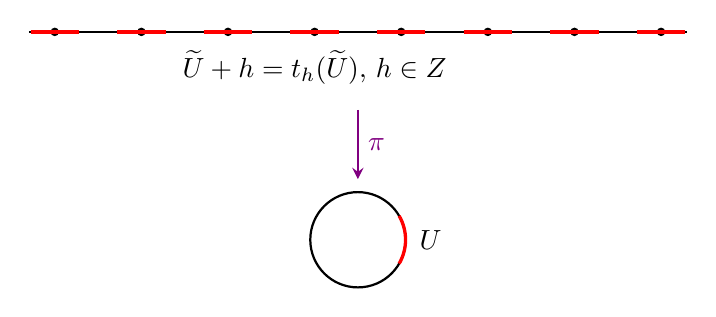
\begin{tikzpicture}[scale=1.1]
        \draw[thick] (-0.3,0) -- (7.3,0);
        \foreach \x in {0,1,2,3,4,5,6,7} {
            \filldraw (\x,0) circle (1.2pt);
        }
        \foreach \x in {0,1,2,3,4,5,6,7} {
            \draw[red, very thick] (\x-0.28,0) -- (\x+0.28,0);
        }
        \node[below] at (3,-0.1) {$\widetilde{U} + h = t_h(\widetilde{U})$, $h \in \mathbb{Z}$};
        \draw[->, >=stealth, thick, Purple] (3.5,-0.9) -- (3.5,-1.7) node[midway, right] {$\pi$};
        \draw[thick] (3.5,-2.4) circle (0.55);
        \draw[red, very thick] ({3.5+0.55*cos(-30)}, {-2.4+0.55*sin(-30)}) arc (-30:30:0.55);
        \node[right] at (4.1,-2.4) {$U$};
    \end{tikzpicture}
    \caption{I traslati $t_h(\widetilde{U})$ (in rosso) di un piccolo intorno sono disgiunti e vengono tutti ``avvolti'' sullo stesso intorno $U \subset S^1$.}
\end{figure}

\section{Gruppo fondamentale di un quoziente}

Sia $(\widetilde{X}, \pi)$ un rivestimento di $X = \widetilde{X}/G$ (con $G$ ad azione propriamente discontinua), $x_0 \in X$ e $\widetilde{x}_0 \in \pi^{-1}(x_0)$. Abbiamo la seguente corrispondenza biunivoca (teorema centrale sui rivestimenti, con $\pi^{-1}(x_0) = G\widetilde{x}_0$):
\[
\Pi_1(X, x_0) \big/ \pi_*\big(\Pi_1(\widetilde{X}, \widetilde{x}_0)\big) \ \longleftrightarrow\ \pi^{-1}(x_0) = G\widetilde{x}_0 \ \longleftrightarrow\ G, \qquad [\sigma] \mapsto \widetilde{\sigma}(1) = g(\widetilde{x}_0) \mapsto g .
\]
(L'applicazione $g \mapsto g(\widetilde{x}_0)$ da $G$ all'orbita \`e iniettiva: se $g(\widetilde{x}_0) = g'(\widetilde{x}_0)$ allora $g^{-1}g'$ ha un punto fisso e, per la propriet\`a di discontinuit\`a, $g^{-1}g' = \mathrm{Id}$.)

\begin{teo}
Se $\widetilde{X}$ \`e il rivestimento \textbf{universale} di $X = \widetilde{X}/G$, allora l'applicazione
\[
F: \Pi_1(X, x_0) \longrightarrow G, \qquad [\sigma] \longmapsto g, \ \text{ dove } \ \widetilde{\sigma}(1) = g(\widetilde{x}_0),
\]
\`e un \textbf{isomorfismo di gruppi}.
\end{teo}
\begin{proof}
Per il corollario sui rivestimenti universali $F$ \`e una bigezione. Basta provare che \`e un omomorfismo: per ogni $[\sigma], [\tau] \in \Pi_1(X, x_0)$, $F([\sigma][\tau]) = F([\sigma]) \circ F([\tau])$.

Sia $F([\sigma][\tau]) = F([\sigma * \tau]) = h \in G$, cio\`e $h(\widetilde{x}_0) = \widetilde{\sigma * \tau}(1)$. Siano $f, g \in G$ tali che $f(\widetilde{x}_0) = \widetilde{\sigma}(1)$ e $g(\widetilde{x}_0) = \widetilde{\tau}(1)$, dove $\widetilde{\sigma}, \widetilde{\tau}$ sono i sollevamenti di $\sigma, \tau$ uscenti da $\widetilde{x}_0$. Poniamo $\widetilde{\tau}_1 = f \circ \widetilde{\tau}$. Allora:
\begin{enumerate}
    \item $\widetilde{\tau}_1$ \`e un sollevamento di $\tau$ (perch\'e $\pi \circ f = \pi$, quindi $\pi \circ \widetilde{\tau}_1 = \pi \circ \widetilde{\tau} = \tau$) uscente da $f(\widetilde{x}_0) = \widetilde{\sigma}(1)$;
    \item perci\`o $\widetilde{\sigma} * \widetilde{\tau}_1$ \`e ben definito, parte da $\widetilde{x}_0$ e solleva $\sigma * \tau$; per l'unicit\`a del sollevamento, $\widetilde{\sigma} * \widetilde{\tau}_1 = \widetilde{\sigma * \tau}$.
\end{enumerate}
Quindi $h(\widetilde{x}_0) = (\widetilde{\sigma} * \widetilde{\tau}_1)(1) = \widetilde{\tau}_1(1) = f(\widetilde{\tau}(1)) = f(g(\widetilde{x}_0))$. Per l'iniettivit\`a di $g \mapsto g(\widetilde{x}_0)$ (vedi sopra), $h = f \circ g$, cio\`e $F([\sigma][\tau]) = F([\sigma]) \circ F([\tau])$\hfill$\square$
\end{proof}

\begin{coro}
$\Pi_1(T^n) \cong \mathbb{Z}^n$ e, per $n \geqslant 2$, $\Pi_1(\mathbb{R}P^n) \cong \mathbb{Z}_2$.
\end{coro}
\begin{proof}
$\mathbb{R}^n \to T^n = \mathbb{R}^n/\mathbb{Z}^n$ e $S^n \to \mathbb{R}P^n = S^n/\{\pm\mathrm{Id}\}$ ($n \geqslant 2$) sono rivestimenti universali dati da gruppi propriamente discontinui $G \cong \mathbb{Z}^n$ e $G \cong \mathbb{Z}_2$ rispettivamente\hfill$\square$
\end{proof}


% ======== NUOVO (pp. 113-114) ========
\section{Algoritmo per il calcolo di $\Pi_1$}

\textbf{Problema.} Dato uno spazio topologico $X$, determinare $\Pi_1(X)$.

\begin{figure}[H]
    \centering
    \begin{tikzpicture}[node distance=1.0cm and 1.2cm,
        box/.style={draw, rounded corners, align=center, minimum height=0.9cm, text width=4.2cm, fill=gray!8},
        dec/.style={draw, diamond, aspect=2.3, align=center, inner sep=1pt, fill=blue!6},
        fin/.style={draw, rounded corners, fill=green!12, minimum height=0.7cm},
        >=Stealth]
        \node[dec] (d1) {$X$ \`e connesso\\ per archi?};
        \node[box, right=2.6cm of d1] (no1) {\textbf{NO:} si applicano i passi successivi a ciascuna componente connessa per archi di $X$};
        \node[dec, below=1.2cm of d1] (d2) {$\Pi_1(X) = 0$?};
        \node[fin, right=2.6cm of d2] (f1) {FINE};
        \node[box, below=1.2cm of d2] (p3) {Trovare $Y$ con $\Pi_1(Y)$ noto, topologicamente o omotopicamente equivalente a $X$: allora $\Pi_1(X) = \Pi_1(Y)$};
        \node[fin, below=0.8cm of p3] (f2) {FINE};
        \draw[->] (d1) -- node[above] {NO} (no1);
        \draw[->] (d1) -- node[left] {S\`I} (d2);
        \draw[->] (d2) -- node[above] {S\`I} (f1);
        \draw[->] (d2) -- node[left] {NO} (p3);
        \draw[->] (p3) -- (f2);
    \end{tikzpicture}
    \caption{Schema dell'algoritmo per calcolare il gruppo fondamentale.}
\end{figure}

\begin{ejemplo}
Sia $X = \mathbb{R}^2 \setminus \{ x \in \mathbb{R}^2 \mid \|x\| = 1 \ \lor\ \|x\| = 2 \}$ (il piano privato delle due circonferenze centrate nell'origine di raggi $1$ e $2$). Calcoliamo $\Pi_1(X)$.

\begin{center}
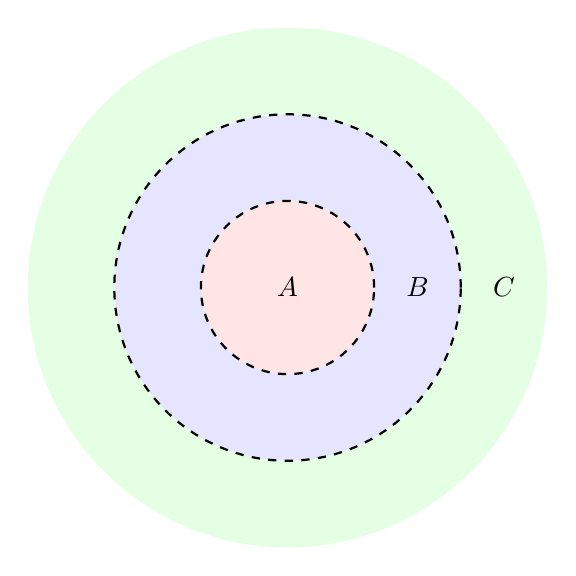
\begin{tikzpicture}[scale=1.1]
    \fill[red!10] (0,0) circle (1);
    \fill[blue!10] (0,0) circle (2); \fill[red!10] (0,0) circle (1);
    \fill[green!10, even odd rule] (0,0) circle (3) (0,0) circle (2);
    \draw[thick, dashed] (0,0) circle (1);
    \draw[thick, dashed] (0,0) circle (2);
    \node at (0,0) {$A$};
    \node at (1.5,0) {$B$};
    \node at (2.5,0.0) {$C$};
\end{tikzpicture}
\end{center}

$X$ \textbf{non} \`e connesso per archi: ha tre componenti connesse per archi:
\[
A = \{\|x\| < 1\}, \qquad B = \{1 < \|x\| < 2\}, \qquad C = \{\|x\| > 2\}.
\]
\begin{itemize}
    \item $\Pi_1(A) = 0$, perch\'e $A$ \`e convesso (un disco aperto \`e contraibile).
    \item $B$ ha come retratto di deformazione la circonferenza $S^1 = \{\|x\| = 3/2\}$ (proiezione radiale), quindi $\Pi_1(B) = \Pi_1(S^1) \cong \mathbb{Z}$. In modo equivalente, $B \cong S^1 \times\, ]1,2[$ e $\Pi_1(S^1 \times\, ]1,2[) \cong \Pi_1(S^1) \times \Pi_1(]1,2[) = \mathbb{Z} \times 0 = \mathbb{Z}$.
    \item $C \cong S^1 \times\, ]0, +\infty[$ ha $S^1$ come retratto di deformazione, quindi $\Pi_1(C) \cong \mathbb{Z}$.
\end{itemize}
Dunque $\Pi_1(A) = 0$, $\Pi_1(B) \cong \Pi_1(C) \cong \mathbb{Z}$ (ciascuna componente va trattata separatamente, con il suo punto base).
\end{ejemplo}

\begin{ejemplo}
Sia $X = S^2 \setminus \gamma$, con $\gamma$ una circonferenza (ad esempio l'equatore). $X$ non \`e connesso per archi: ha due componenti connesse per archi $A$ e $B$ (le due calotte aperte). Ciascuna \`e omeomorfa a un disco aperto $\mathring{B}^2$ (per proiezione), quindi contraibile: $\Pi_1(A) = \Pi_1(B) = 0$.
\end{ejemplo}

\begin{ejemplo}
Sia $X = \mathbb{R}^3 \setminus r$, con $r$ una retta. $X$ \`e connesso per archi e $\Pi_1(X) \neq 0$: un cappio che gira attorno alla retta non si pu\`o contrarre al cappio costante (la retta \`e infinita, non c'\`e modo di ``sfilare'' il cappio). Per calcolarlo:
\begin{itemize}
    \item \textbf{Metodo 1.} Un cilindro infinito $\mathscr{C} = S^1 \times \mathbb{R}$ avente $r$ come asse (privato dell'asse) \`e un retratto di deformazione di $X$ (si spinge ogni punto radialmente sul cilindro), quindi $\Pi_1(X) = \Pi_1(S^1 \times \mathbb{R}) = \Pi_1(S^1) \times \Pi_1(\mathbb{R}) = \mathbb{Z}$.
    \item \textbf{Metodo 2.} Si pu\`o prendere un piano ortogonale a $r$ che interseca $r$ in un punto $p$: $\mathbb{R}^3 \setminus r$ si retrae per deformazione su $\mathbb{R}^2 \setminus \{p\}$. Quindi $\Pi_1(X) = \Pi_1(\mathbb{R}^2 \setminus \{p\}) = \Pi_1(S^1) = \mathbb{Z}$.
\end{itemize}
\end{ejemplo}

\begin{figure}[H]
    \centering
    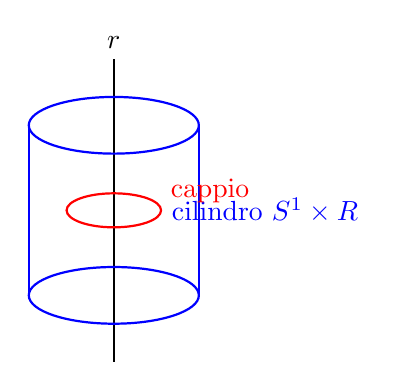
\begin{tikzpicture}[scale=1.2]
        \draw[thick] (0,-1.6) -- (0,1.6) node[above] {$r$};
        \draw[blue, thick] (0,0.9) ellipse (0.9 and 0.3);
        \draw[blue, thick] (0,-0.9) ellipse (0.9 and 0.3);
        \draw[blue, thick] (-0.9,0.9) -- (-0.9,-0.9);
        \draw[blue, thick] (0.9,0.9) -- (0.9,-0.9);
        \node[blue] at (1.6,0) {cilindro $S^1\times\mathbb{R}$};
        \draw[red, thick, ->, >=stealth] (0,0) ellipse (0.5 and 0.18);
        \node[red, right] at (0.5,0.2) {cappio};
    \end{tikzpicture}
    \caption{$\mathbb{R}^3 \setminus r$ si retrae per deformazione su un cilindro che ha $r$ come asse; il cappio attorno a $r$ genera $\Pi_1 = \mathbb{Z}$.}
\end{figure}

\begin{ejemplo}
Sia $X = \mathbb{R}^2 \setminus (S^1 \cup \{p\})$, con $S^1$ la circonferenza unitaria e $p$ un punto. Ci sono due configurazioni possibili.

\begin{center}
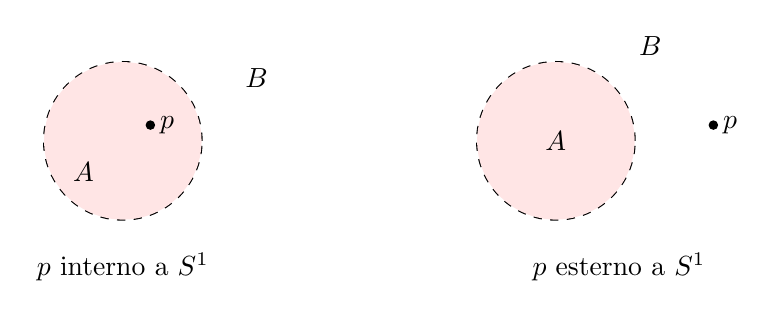
\begin{tikzpicture}[scale=1.0]
    % p interno
    \begin{scope}
        \draw[thick, dashed] (0,0) circle (1);
        \fill[red!10] (0,0) circle (1);
        \filldraw (0.35,0.2) circle (1.5pt) node[right] {$p$};
        \node at (-0.5,-0.4) {$A$}; \node at (1.7,0.8) {$B$};
        \node[below] at (0,-1.3) {$p$ interno a $S^1$};
    \end{scope}
    % p esterno
    \begin{scope}[shift={(5.5,0)}]
        \draw[thick, dashed] (0,0) circle (1);
        \fill[red!10] (0,0) circle (1);
        \filldraw (2.0,0.2) circle (1.5pt) node[right] {$p$};
        \node at (0,0) {$A$}; \node at (1.2,1.2) {$B$};
        \node[below] at (0.8,-1.3) {$p$ esterno a $S^1$};
    \end{scope}
\end{tikzpicture}
\end{center}

\begin{enumerate}
    \item \textbf{$p$ interno alla circonferenza.} $X$ non \`e connesso per archi e ha due componenti $A$ (il disco aperto privato di $p$) e $B$ (la parte esterna al disco). $\Pi_1(A) \neq 0$ (un cappio attorno a $p$ non si contrae); $A$ ha $S^1$ come retratto di deformazione, quindi $\Pi_1(A) = \Pi_1(S^1) = \mathbb{Z}$; e $\Pi_1(B) = \mathbb{Z}$ (gi\`a visto).
    \item \textbf{$p$ esterno alla circonferenza.} Ancora due componenti: $A$ \`e il disco aperto, quindi $\Pi_1(A) = 0$; $B$ \`e l'esterno del disco privato di $p$ e $\Pi_1(B) \neq 0$ (un cappio attorno al disco, o attorno a $p$, non si contrae). Osserviamo che $S^1 \vee S^1$ \`e un retratto di deformazione di $B$ (il piano privato di un disco chiuso e di un punto ha lo stesso tipo di omotopia del piano privato di due punti), quindi
    \[
    \Pi_1(B) = \Pi_1(S^1 \vee S^1) = F_2 .
    \]
\end{enumerate}
\end{ejemplo}


